\documentclass[11pt]{article}
\usepackage[a4paper,margin=1in]{geometry}
\reversemarginpar
\usepackage{mathtools, amsthm, amssymb, amsmath}
\usepackage{multicol}
\usepackage{hyperref}
\usepackage{subcaption}
\usepackage{longtable}
\usepackage{graphicx}
\graphicspath{{./picture/}}
\usepackage{subcaption}
\usepackage{tikz}
\usetikzlibrary{positioning}
\usepackage{rotating}
\usepackage{mfirstuc}
\usepackage[backend=biber, style=ieee]{biblatex}
\addbibresource{MV.bib}
%\usepackage{todonotes}


\newtheorem{theorem}{Theorem}[section]
\theoremstyle{definition}
\newtheorem{definition}[theorem]{Definition}
\newtheorem{example}[theorem]{Example}

\DeclareMathOperator{\dom}{dom}

\title{Generating Music Variations through Chaotic Dynamical Systems Exploration}
\author{Rajamangala University of Technology Thanyaburi\\Kanatsanun Sub-udom\\Wannasa Rianthong\\Patipan Somwong}


\begin{document}
\maketitle
\begin{abstract}
This paper proposes a novel approach to introducing variation in musical compositions, addressing the challenge of composer burnout. 
By exploiting the properties of chaotic dynamical systems, renowned for their sensitivity to initial conditions, this method combines melodic variation with an expanded rhythmic structure. 
The rhythmic expansion is achieved through prolonging the duration of musical notes, leading to a seamless integration of melodic and rhythmic elements. 
The technique involves mapping musical data onto a chaotic attractor, generating new variations as the system's trajectories evolve. 
The aim is to provide composers with a systematic and creative tool for exploring fresh musical ideas, alleviating creative fatigue, and reinvigorating the compositional process.
\end{abstract}

\section{Introduction}
Music variation serves as a catalyst for creative thinking in the songwriting process. It offers flexibility, capable of generating patterns ranging from close replicas to entirely different ones. The outcome depends on the composer's desires. When applied to compositions, it's like creating another version of the same song, making the music open to change every time it's heard. In the past, composers often employed techniques like inversion, retrograde or sections of music to expand upon the original musical content. However, these techniques gradually lost their appeal and were seen as tiresome. Music variation steps in to fill this gap. This technique opens up possibilities for composers to create entirely new musical patterns without being tied to the original framework. Individuals can transform the written notes into their own unique dynamic and fresh music.

Nowadays, artificial intelligence (AI) technologies have significantly advanced, enabling them to create music with ever-increasing proficiency \cite{bonnici_music_2021}. 
Well-known AI music generation platforms such as Mubert \cite{mubert_website} and 
Musicity \cite{musicfy_website} empower users with real-time music generation capabilities, 
enabling them to effortlessly select their preferred genre or mood and promptly receive a personalized soundtrack tailored to their preferences. On the other hand, Soundraw \cite{soundraw_website} and Boomy \cite{boomy_website} function as AI-driven music creation tools, furnishing a diverse array of features to aid users in sculpting their musical opuses with ease. Meanwhile, AIVA \cite{aiva_website} harnesses the power of deep learning to craft original music closely resembling the distinctive style of a particular artist or genre. Users can furnish reference tracks or articulate their desired musical aesthetics, prompting AIVA to generate fresh compositions that align precisely with their specifications. However, these technologies often require high computational resources, making them unable to run on devices with low processing power. Additionally, some AI music composition tools may produce music in limited styles.

Since limitations of AI music technology is an expensive problem to leave unaddressed, the following consequences it may lead to. Firstly, aspiring artists and musicians will miss out on the opportunity to use these tools due to limited access, as most people lack high-performance equipment. Furthermore, all music generated by AI may start to sound similar, potentially leading to a lack of musical diversity. The paper thus aims to address the aforementioned issue by employing a multi-step process. Initially, it utilizes melodic variation with expanded rhythm, which is then translated into numerical values. These numerical values are then input into a chaotic dynamical system, resulting in a new set of numbers different from the original. Finally, these numbers are mapped back to musical notes, resulting in the creation of a new piece of music. This method requires lower computing resources compared to using AI music composition technology and allows for the creation of diverse musical compositions depending on the original song, initial values, and equations used.

The paper is structured as follows. Section \ref{sec: literaturereview} provides an overview of relevant mathematical notations and music theory concepts. 
The main result is presented in Section \ref{sec: mainresult}, where we propose techniques involving chaotic dynamical systems to generate new variations in musical pitch. 
Additionally, we employ melodic variation with expanded rhythm for each pitch, creating music that significantly differs from the first method. 
Section \ref{sec: discussion} discusses the strengths and weaknesses of the combined musical variations resulting from the chaotic mapping and melodic variation with expanded rhythm methods, along with limitations, considerations, and future directions. 
Finally, the last section summarizes the solutions and insights derived to address the issues discussed in the paper succinctly and conclusively.

\section{Literature Review}
\label{sec: literaturereview}

Throughout this paper, we use the following notation. Denote $\mathbb{R}$ the set of real numbers, $\mathbb{N}$ the set of natural numbers and $\mathbb{R}_{+}$ the set of positive real numbers. For any fixed $n \in \mathbb{N}$, we denote $\mathbb{N}_n := \{ 1, 2, \dots, n \}$, $\mathbb{R}^n$ the $n$-dimensional euclidean space and $\{ a_k \}_{k=0}^{n} = \{ a_0, a_1, \dots, a_n \}$ a sequence of real numbers. Denote $ \left\lVert x \right\rVert$ the euclidean norm of vector $x$. A function $f$ is injective if $f(x_1) = f(x_2)$ implies $x_1 = x_2$. Denote $\dom{f}$ the domain of the function $f$. 
A dynamical system
\begin{equation} \label{eq: lrdotx}
\dot{x}(t) = f(t, x)
\end{equation} 
is composed through a system of ordinary differential equations, where $\dot{x}(t)$ represents the derivative of $x(t)$ with respect to time. 
The point $x^* \in \mathbb{R}^n$ is called an equilibrium point of the system \eqref{eq: lrdotx} if $f(t, x^*) = 0 $ for all $t \geq 0$.

In music theory, a musical note is a symbol on a staff that represents pitch, which refers to the highness or lowness of a sound. Notes are typically represented by the letters A through G, corresponding to the solfege syllables (Do, Re, Mi, Fa, Sol, La, Ti). Musical notation also incorporates numbers to specify the precise pitch of a musical note. As shown in Figure \ref{fig:musical note}, there are two sets of five horizontal lines, known as the treble clef (the top set of lines) and the bass clef (the bottom set of lines).
The treble clef is used to represent higher pitches, while the bass clef is used to represent lower pitches. Each line and space on the staff corresponds to a specific pitch. For example, the note C4, indicated in Figure \ref{fig:musical note}, is lower in pitch than the note D4, which is located on the line above it.
Similarly, the note C6, shown above the treble clef in Figure \ref{fig:musical note}, represents a higher pitch than the note C5, which is located on the second-highest line of the treble clef. Therefore, notes higher on the staff represent higher pitches, and notes lower on the staff represent lower pitches.
It is important to note that the pitches represented on the treble clef are generally higher than those represented on the bass clef. For instance, the note C5 (located on the treble clef) has a higher pitch than the note B4 (located on the bass clef). 
Additionally, each musical note has a duration symbol that specifies how long it should be played. Durations are typically defined using the unit beat, which refers to a chosen time interval. For example, if we establish from a duration table, see Figure \ref{tab:note duration}, that 1 beat is equivalent to playing a musical note for 1 second, then 2 beats would correspond to playing a note for 2 seconds. For convenience, we can establish a general rule: let t beats equal playing a musical note for t seconds, where t is any positive number. This rule allows us to understand the meaning of fractional beats. For instance, 0.5 beats would signify playing a musical note for 0.5 seconds. This example emphasizes that the relationship of t beats to playing a note for t seconds is a common way to explain the fundamental concept of musical note durations. 

\begin{figure}
\centering
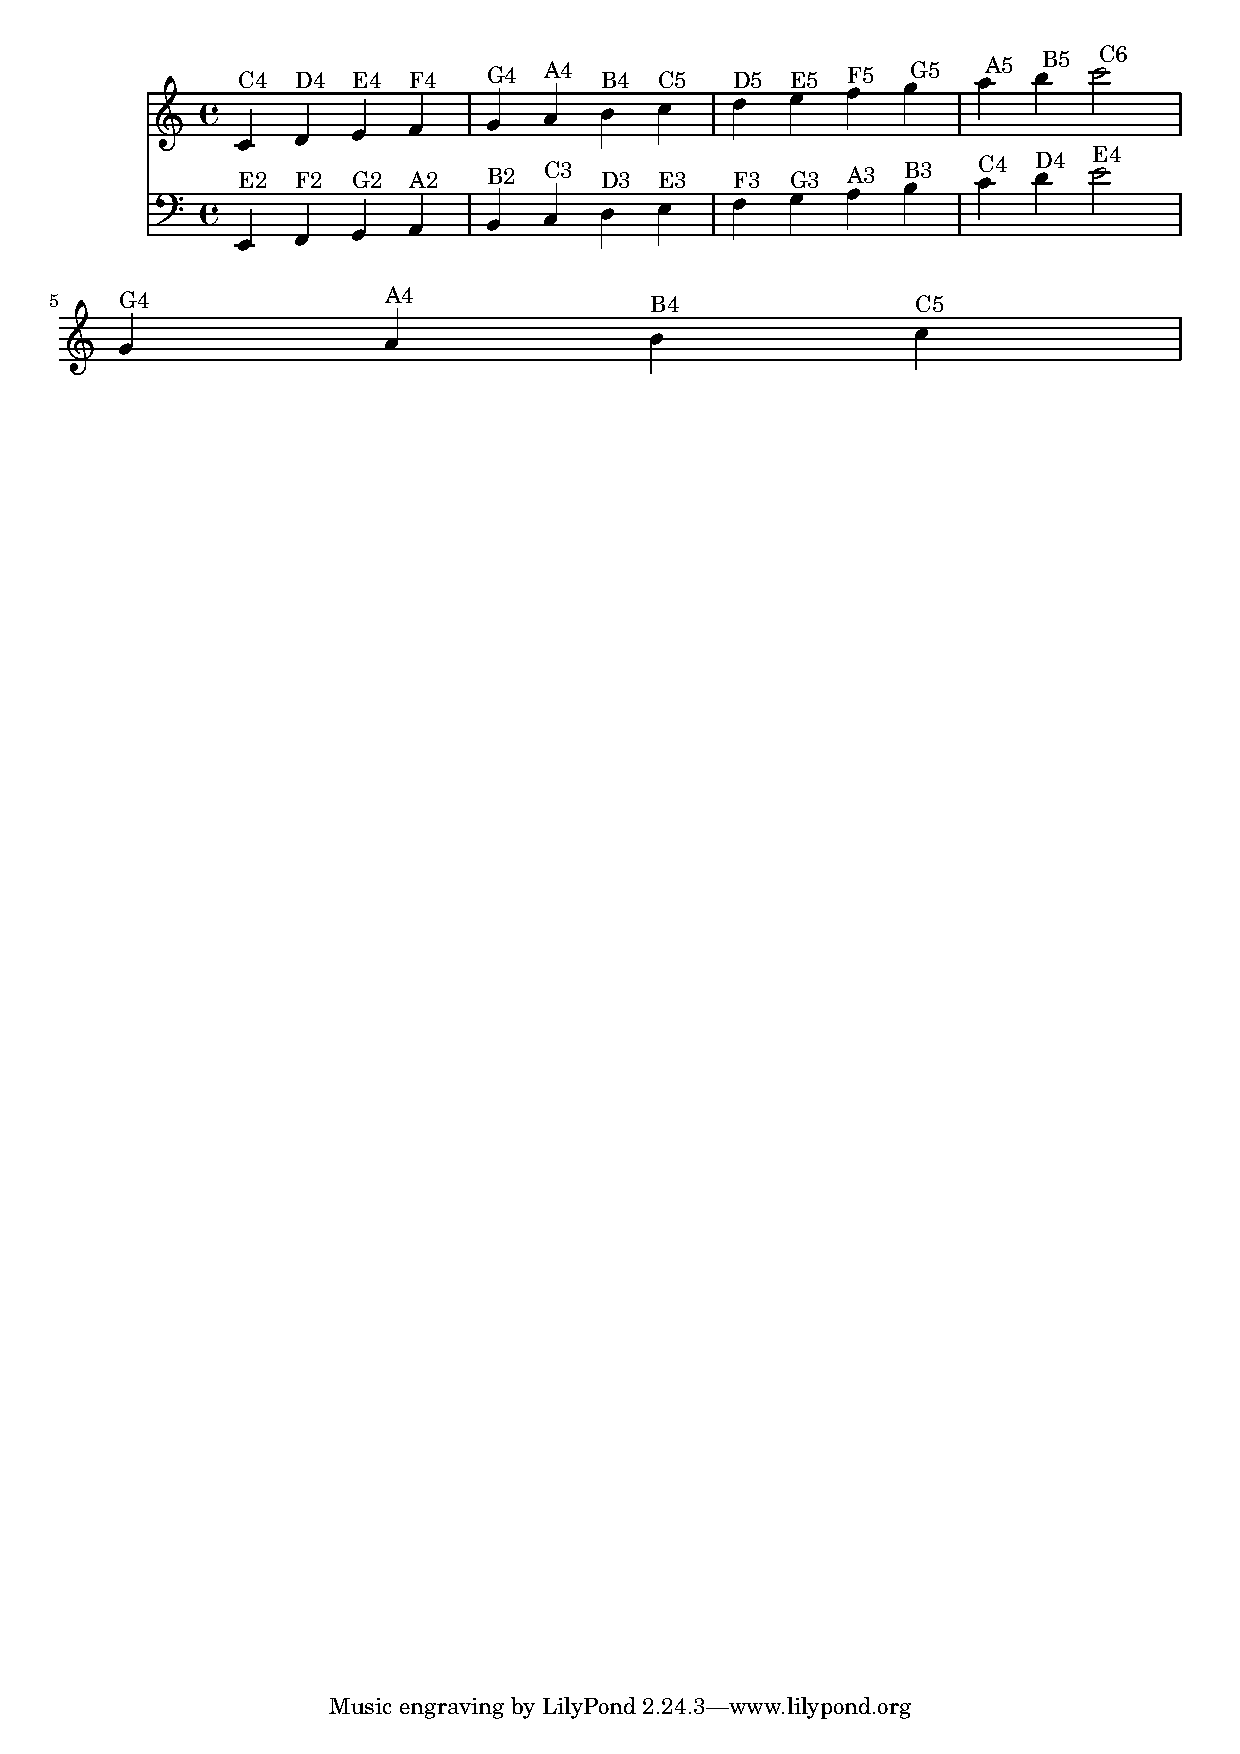
\includegraphics[trim=1cm 25cm 0cm 0.02cm, clip, scale=0.8]{pitchesonstaff.pdf} % trim={left bottom right top}
\caption{Musical notes ranging from E2 to C6.}
\label{fig:musical note} 
\end{figure}

\begin{table}
\centering
\begin{tabular}{|c|c|c|}
\hline
\textbf{Musical Note} & \textbf{Duration (Beat)} \\
\hline
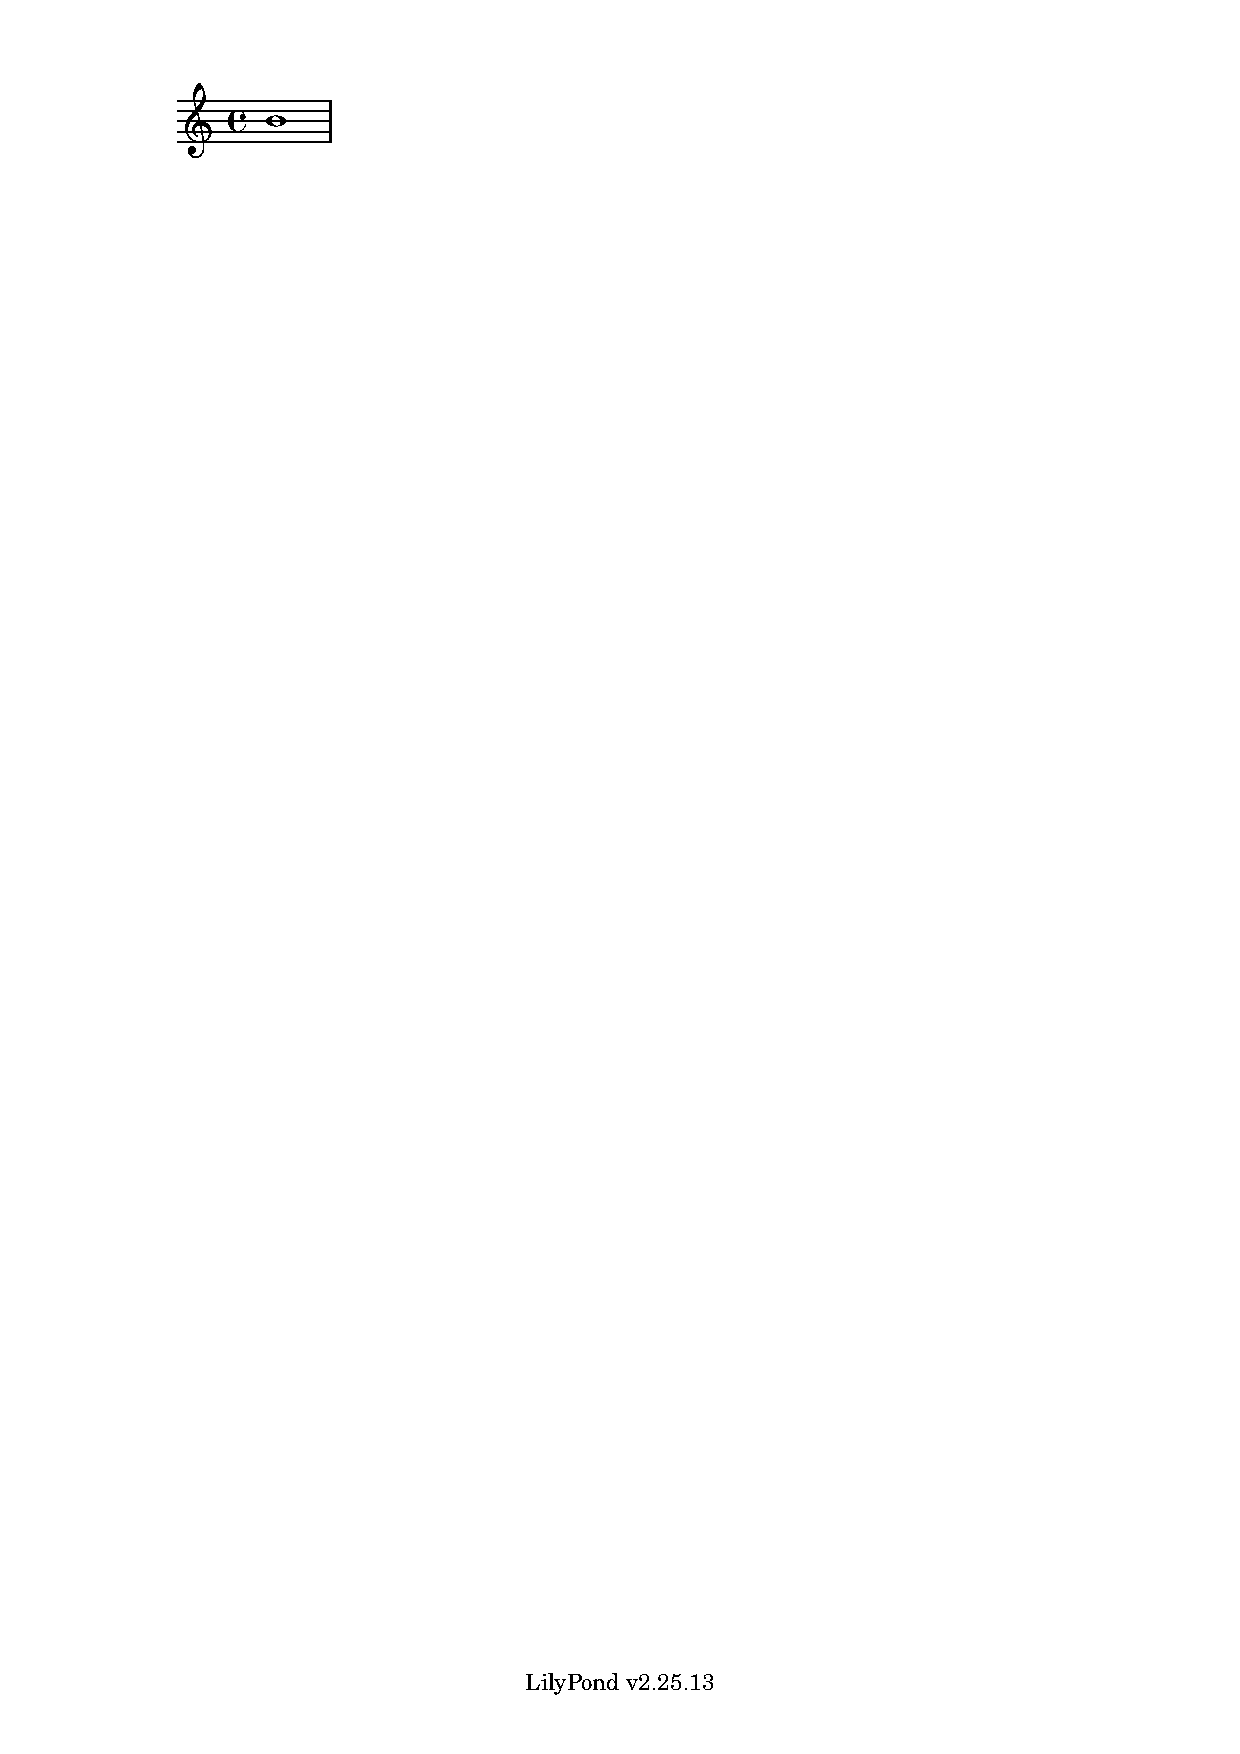
\includegraphics[trim=4.29cm 27.25cm 16cm 1.5cm, clip, scale=1]{whole_note.pdf} & 4  \\
\hline
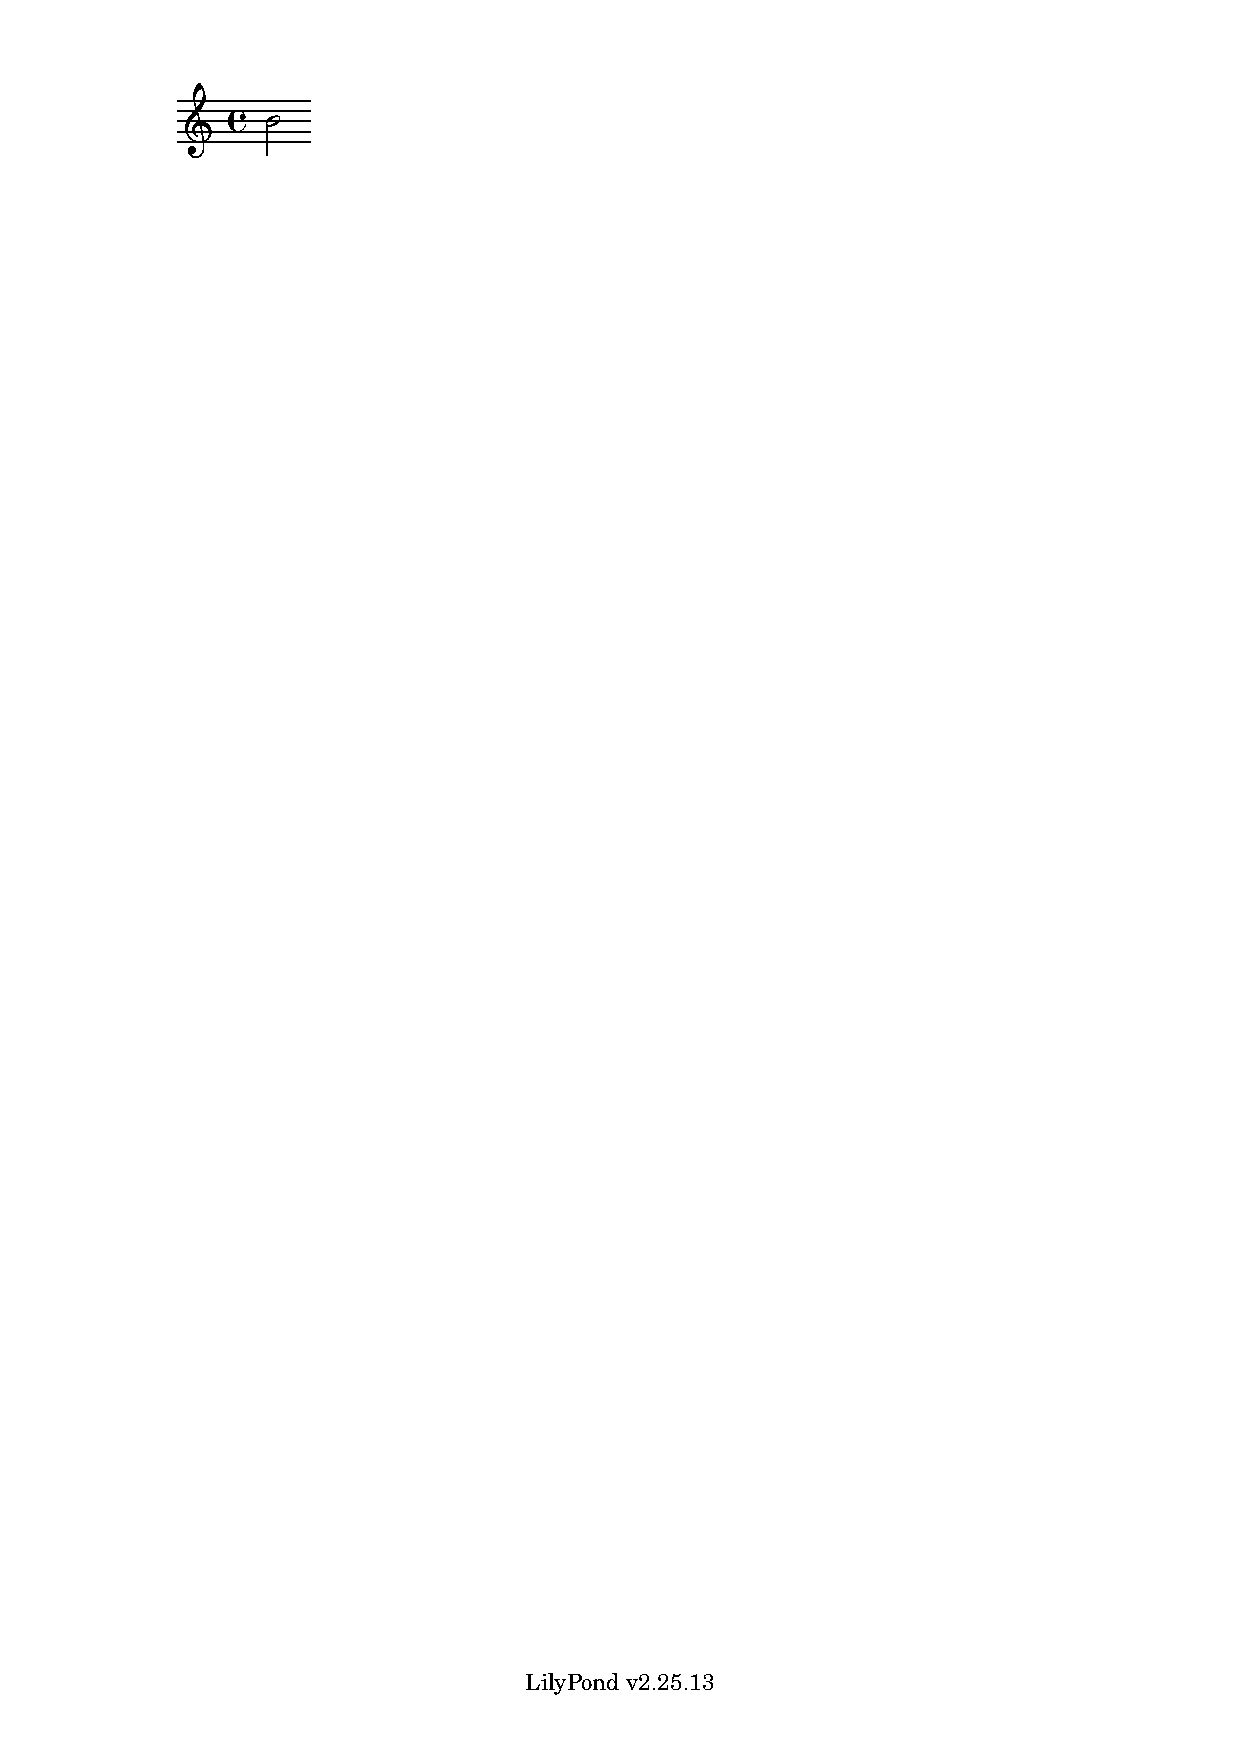
\includegraphics[trim=4.29cm 27cm 16cm 1.5cm, clip, scale=1]{half_note.pdf} & 2  \\
\hline
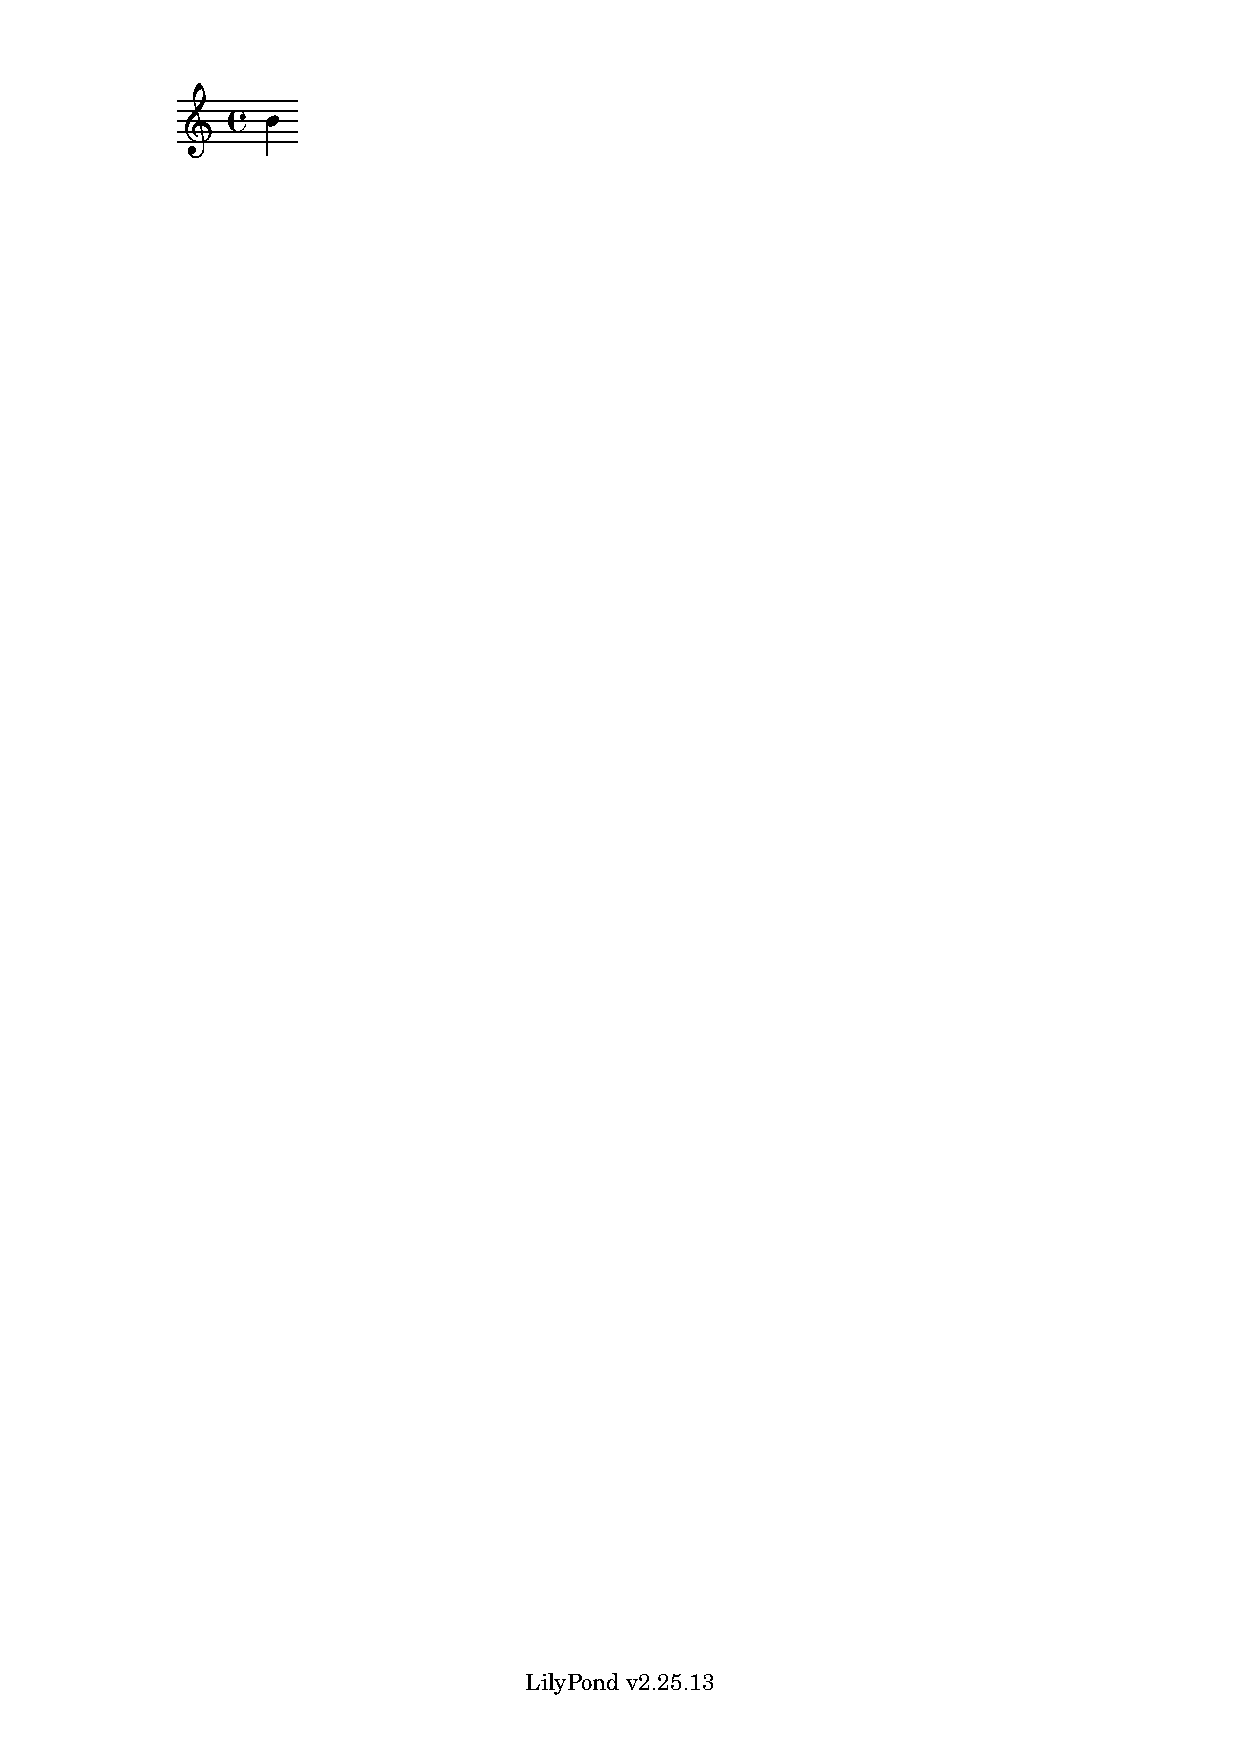
\includegraphics[trim=4.29cm 27cm 16cm 1.5cm, clip, scale=1]{quarter_note.pdf} & 1 \\
\hline
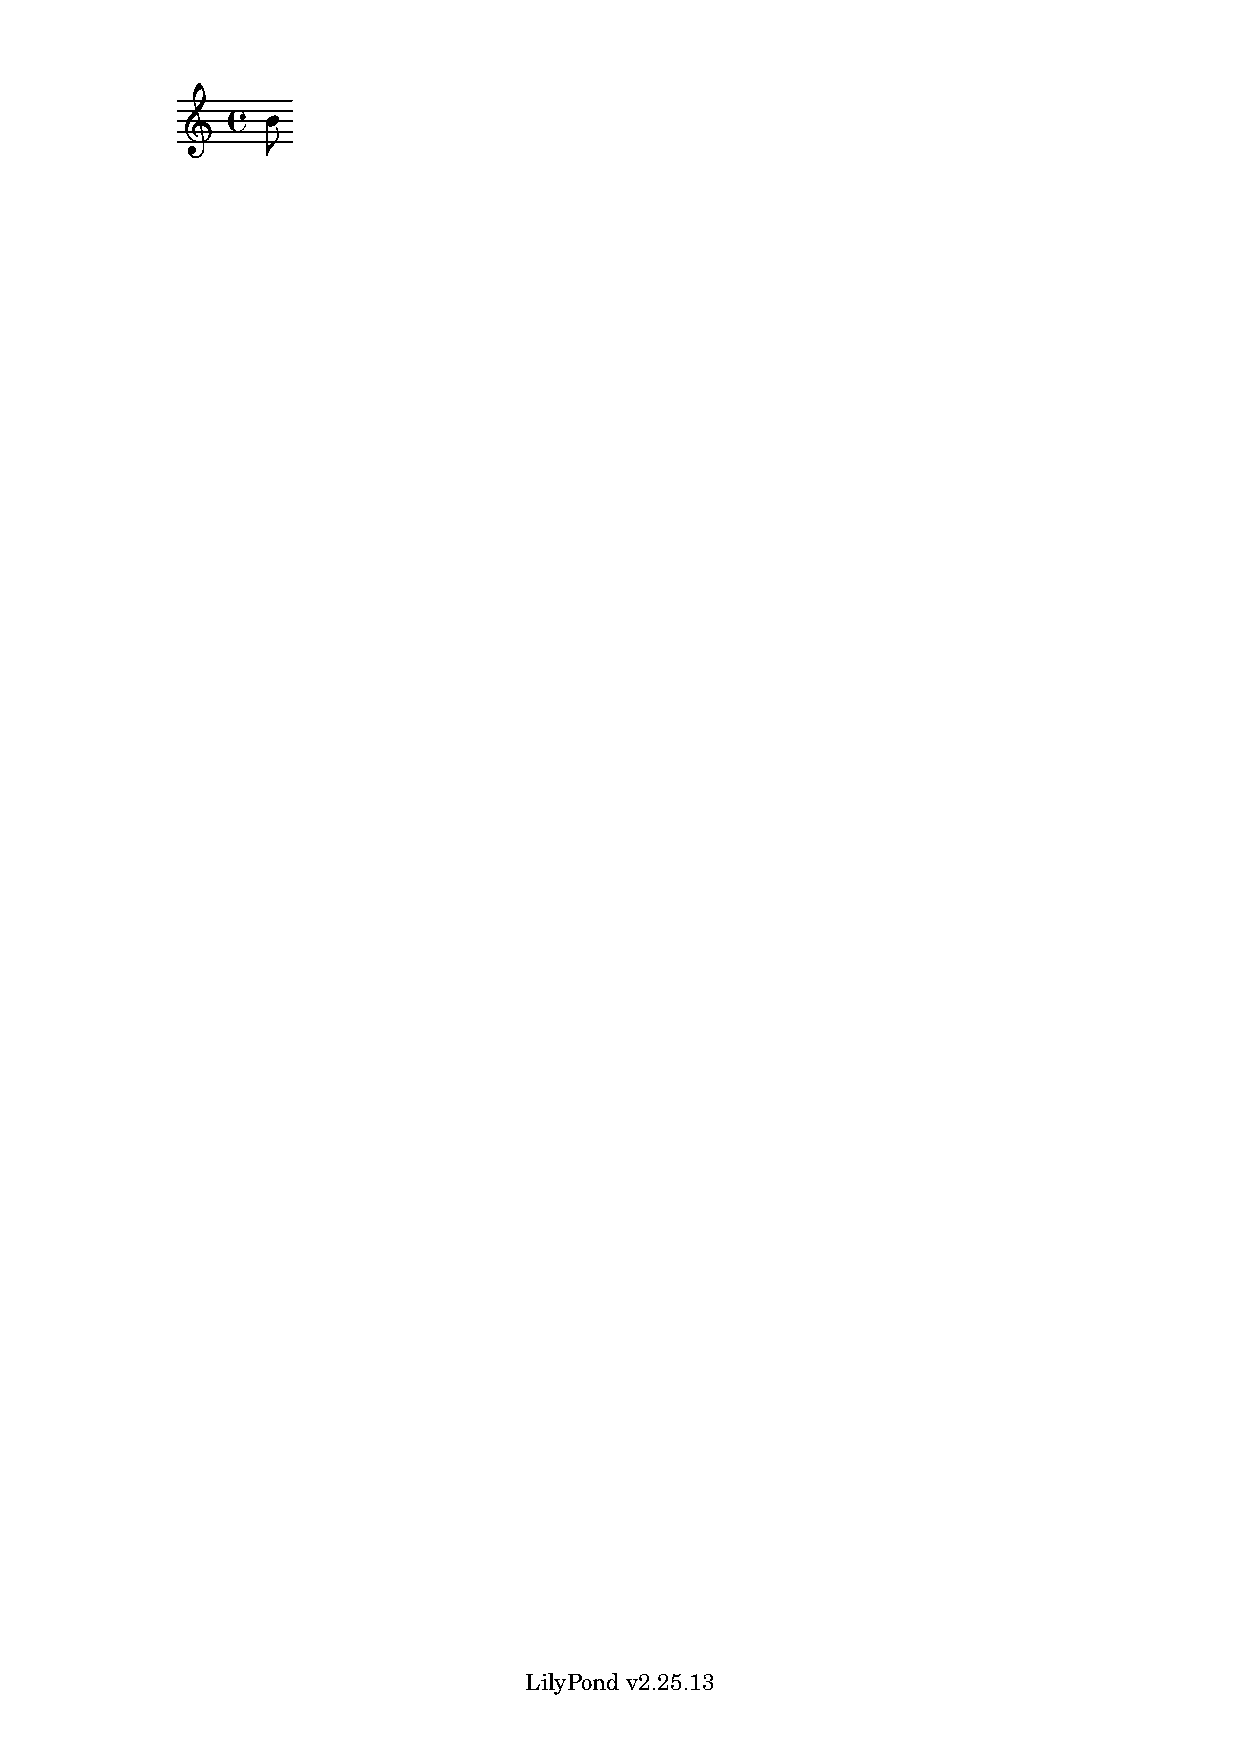
\includegraphics[trim=4.29cm 27cm 16cm 1.5cm, clip, scale=1]{eighth_note.pdf} & 1/2 \\
\hline
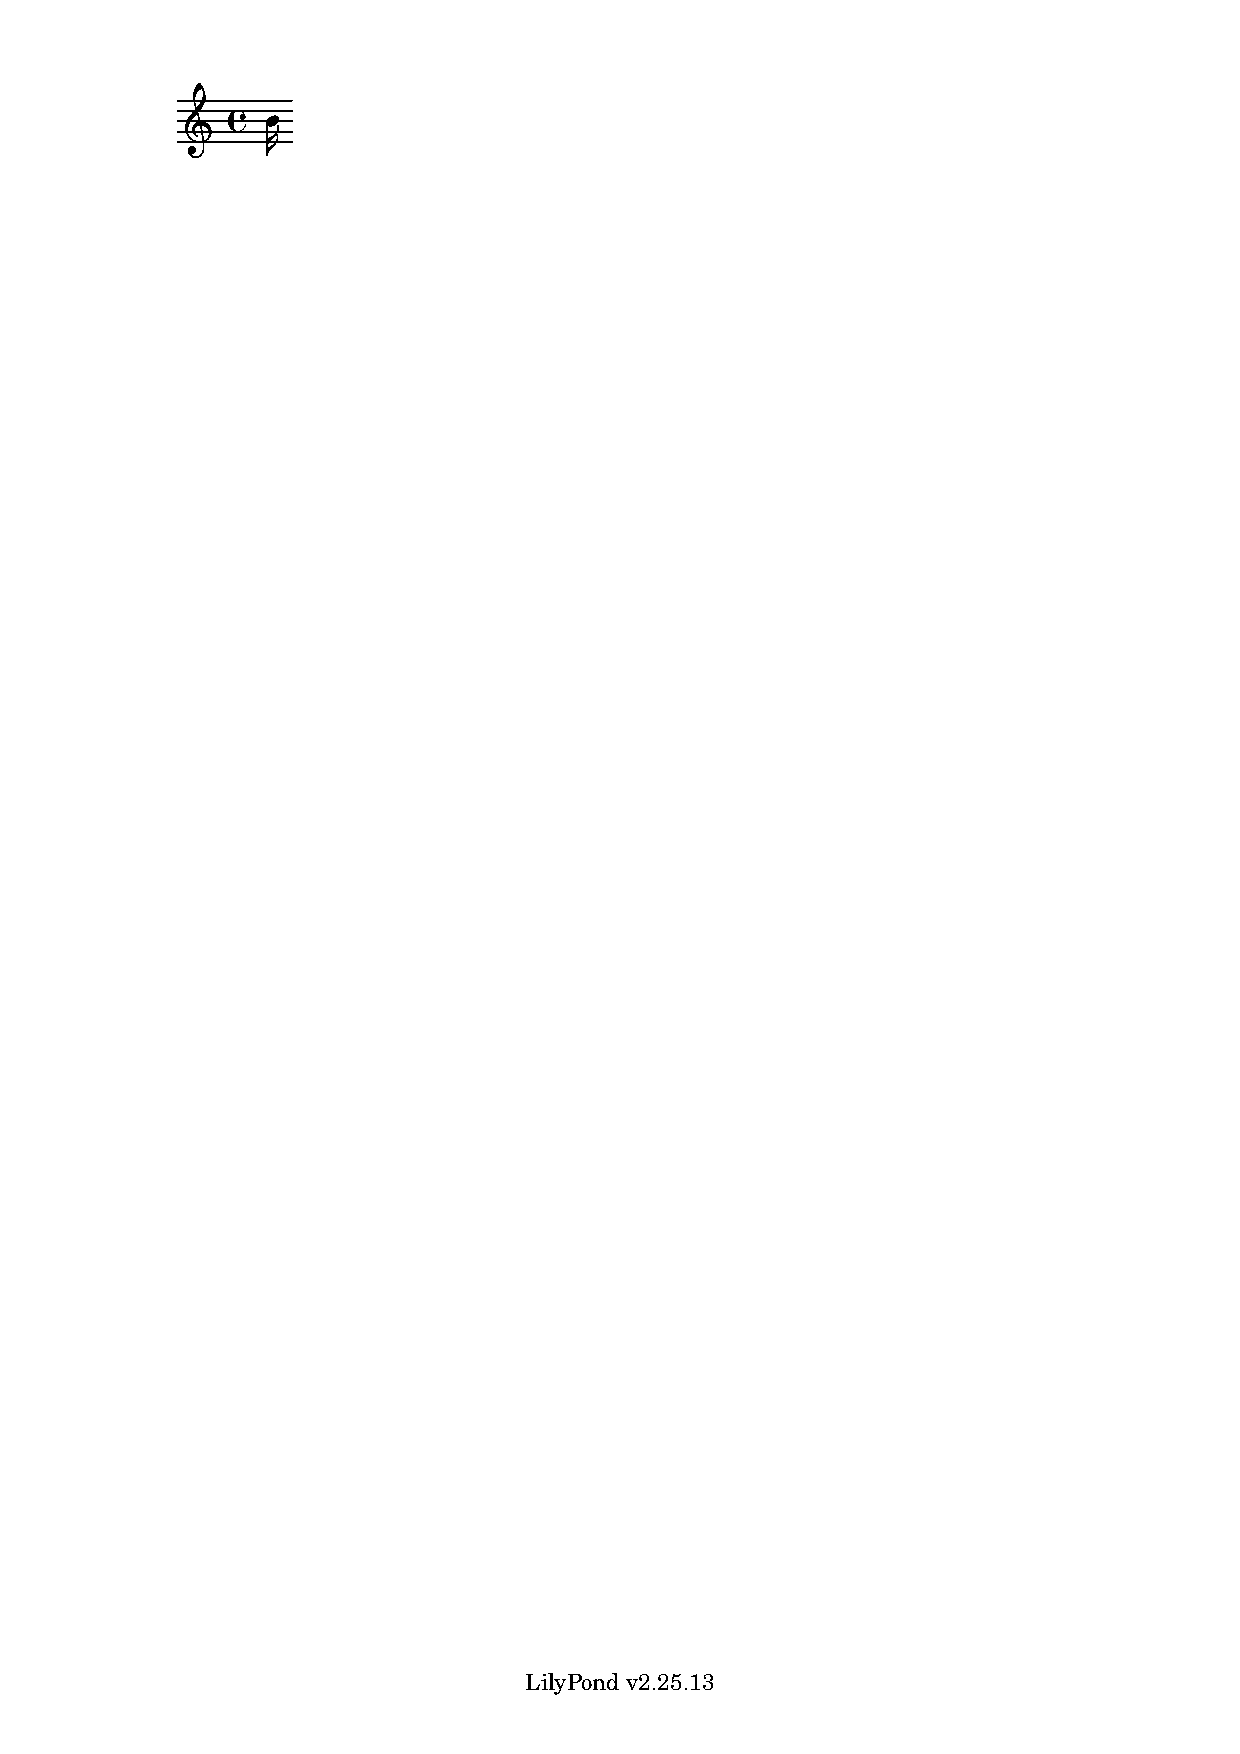
\includegraphics[trim=4.29cm 27cm 16cm 1.5cm, clip, scale=1]{sixteenth_note.pdf} & 1/4 \\
\hline
\end{tabular}
\caption{Duration of musical notes and their corresponding beats}
\label{tab:note duration}
\end{table}

Recent advancements in the study of chaotic systems have sparked significant interest in designing systems with diverse characteristics. These systems range from those devoid of equilibrium point \cite{ren_new_2018,wang_s-box_2019} to those with only one stable equilibrium \cite{wang_chaotic_2011}, two stable equilibria \cite{wang_chaotic_2017}, multi-scroll attractors \cite{rajagopal_multiscroll_2019,pehlivan_multiscroll_2019}, various types of symmetry \cite{field_symmetry_2009}. There are also uses of memristors, memcapacitors, cubic nonlinear resistors, and piecewise linear functions as nonlinear factors to create chaos \cite{article,varan_control_2018,rajagopal_dynamical_2019,akgul_chaotic_2019,rajagopal_simple_2019}.
A chaotic system is characterized by three fundamental properties essential for comprehending its behavior. Firstly, Aperiodic long-term behavior means these systems never settle into predictable patterns. Unlike regular systems that eventually reach an equilibrium point, chaotic systems constantly change and never truly repeat themselves. Secondly, chaotic systems are deterministic, meaning their complex behavior arises solely from the internal interactions within the system, without any random inputs or external noise. This inherent nonlinearity within the system is what creates the seemingly unpredictable movements, not chance. Thirdly, its sensitive dependence on initial conditions highlights how even the slightest difference in starting conditions can lead to completely different outcomes. Imagine a tiny change in the starting conditions causing the system to behave wildly differently, like a butterfly flapping its wings causing a hurricane. These defining traits of chaos have found extensive applications across various disciplines. However, despite their broad recognition, universally acknowledged theories elucidating these phenomena may still prove elusive. For example, these properties are often applied to chaotic systems employed in modeling natural phenomena \cite{jan_dynamical_2022}, exemplified by their capacity to elucidate various natural phenomena, including weather patterns \cite{knight_metlink_2021}, turbulent fluid flows \cite{turbulent}, ecological systems \cite{crawford_ecological_2020}, and population dynamics \cite{jung_chaotic_2020}. In the domain of finance and economics \cite{liao_study_2020}, scholars investigate chaotic dynamics to model stock market fluctuations \cite{vogl_chaos_2024}, economic cycles \cite{tusset_dynamic_2023}, and price dynamics \cite{ait_omar_chaotic_2022}, thereby providing insights into the intrinsic unpredictability and nonlinear behavior inherent in financial systems. Likewise, within biomedical systems \cite{korolj_healthy_2019}, chaotic systems assume a pivotal role in the modeling and comprehension of intricate biological systems \cite{li_incorporating_2023}, encompassing neural networks \cite{lin_chaotic_2020}, cardiac rhythms \cite{cheffer_biochaos_2022}, and gene regulatory networks \cite{uthamacumaran_review_2021}. The Belousov-Zhabotinsky, a chaotic system exhibiting spiral wave patterns from its nature, can create cellular automata models with complex behavior based on reactant concentrations and temperature \cite{karimov_empirically_2023,luengviriya_meandering_2013,chopard_cellular_2022}.

One of the well-known chaotic systems is the Lorenz system \cite{Lorenz}, a dynamical system with parameters $\sigma > 0$, $r > 0$ and $b > 0$ given by:
\begin{equation} \label{eq: lorenz}  
\begin{aligned}
\dot{x}_1 &= \sigma(x_2 - x_1), \\
\dot{x}_2 &= rx_1 - x_2 - x_1x_3, \\
\dot{x}_3 &= x_1x_2 - bx_3.
\end{aligned}
\end{equation}
The system \eqref{eq: lorenz} is nonlinear due to the presence of terms like $x_1x_2$ and $x_1x_3$ in the equations, indicating that the variables interact in a complex complex way. Moreover, it has equilibrium point at $(x^*_1, x^*_2, x^*_3) = (0, 0, 0)$ for all parameter values. Additionally, for $r > 1$ there exist two additional equilibrium points at $x^*_1 = x^*_2 = \pm \sqrt{b(r - 1)}$, $x^*_3 = r-1$. 
For an instance, if parameters set to $\sigma = 10$, $r = 28$ and $b = \dfrac{8}{3}$, it exhibits chaotic behavior, as illustrated in Figure \ref{fig:LE}. The figure shows the aperiodic long-term behavior, its deterministic nature and its sensitive dependence on initial conditions.

\begin{figure}
\centering
\begin{subfigure}{0.45\textwidth}
  \centering
  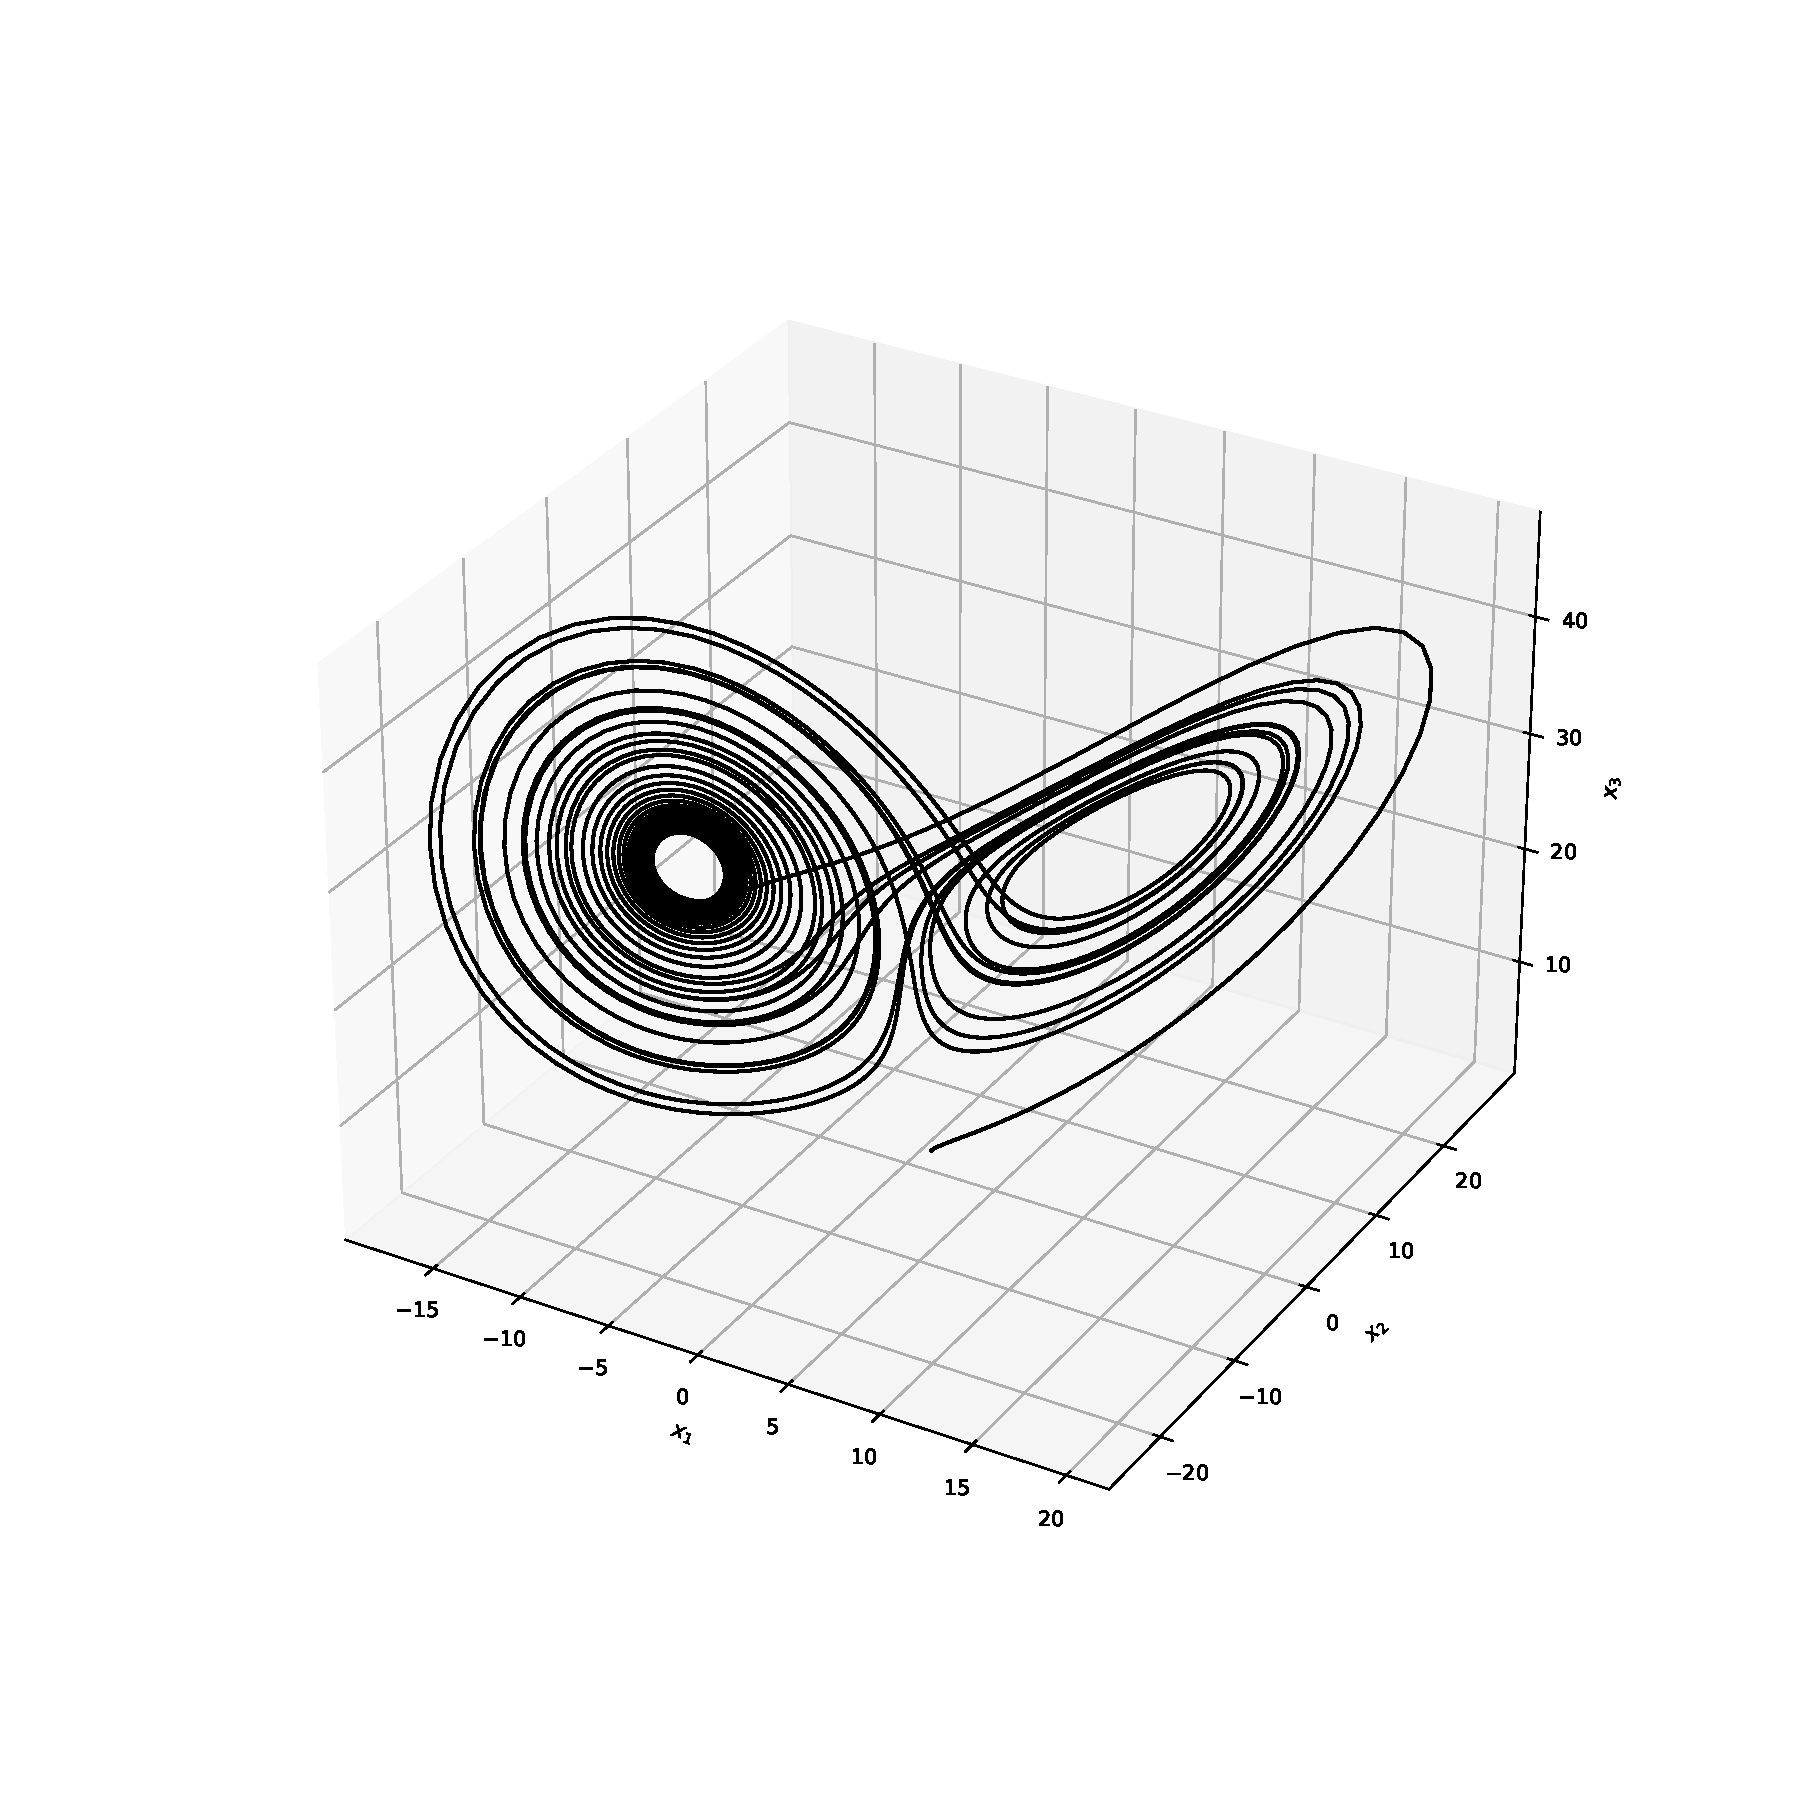
\includegraphics[trim=2cm 2cm 2cm 2cm, clip, scale=0.3]{Lorenz1.pdf}
  \caption{Initial condition $(1,1,1)$.}
  \label{subfig1:mp}
\end{subfigure}\hfill
\begin{subfigure}{0.45\textwidth}
  \centering
  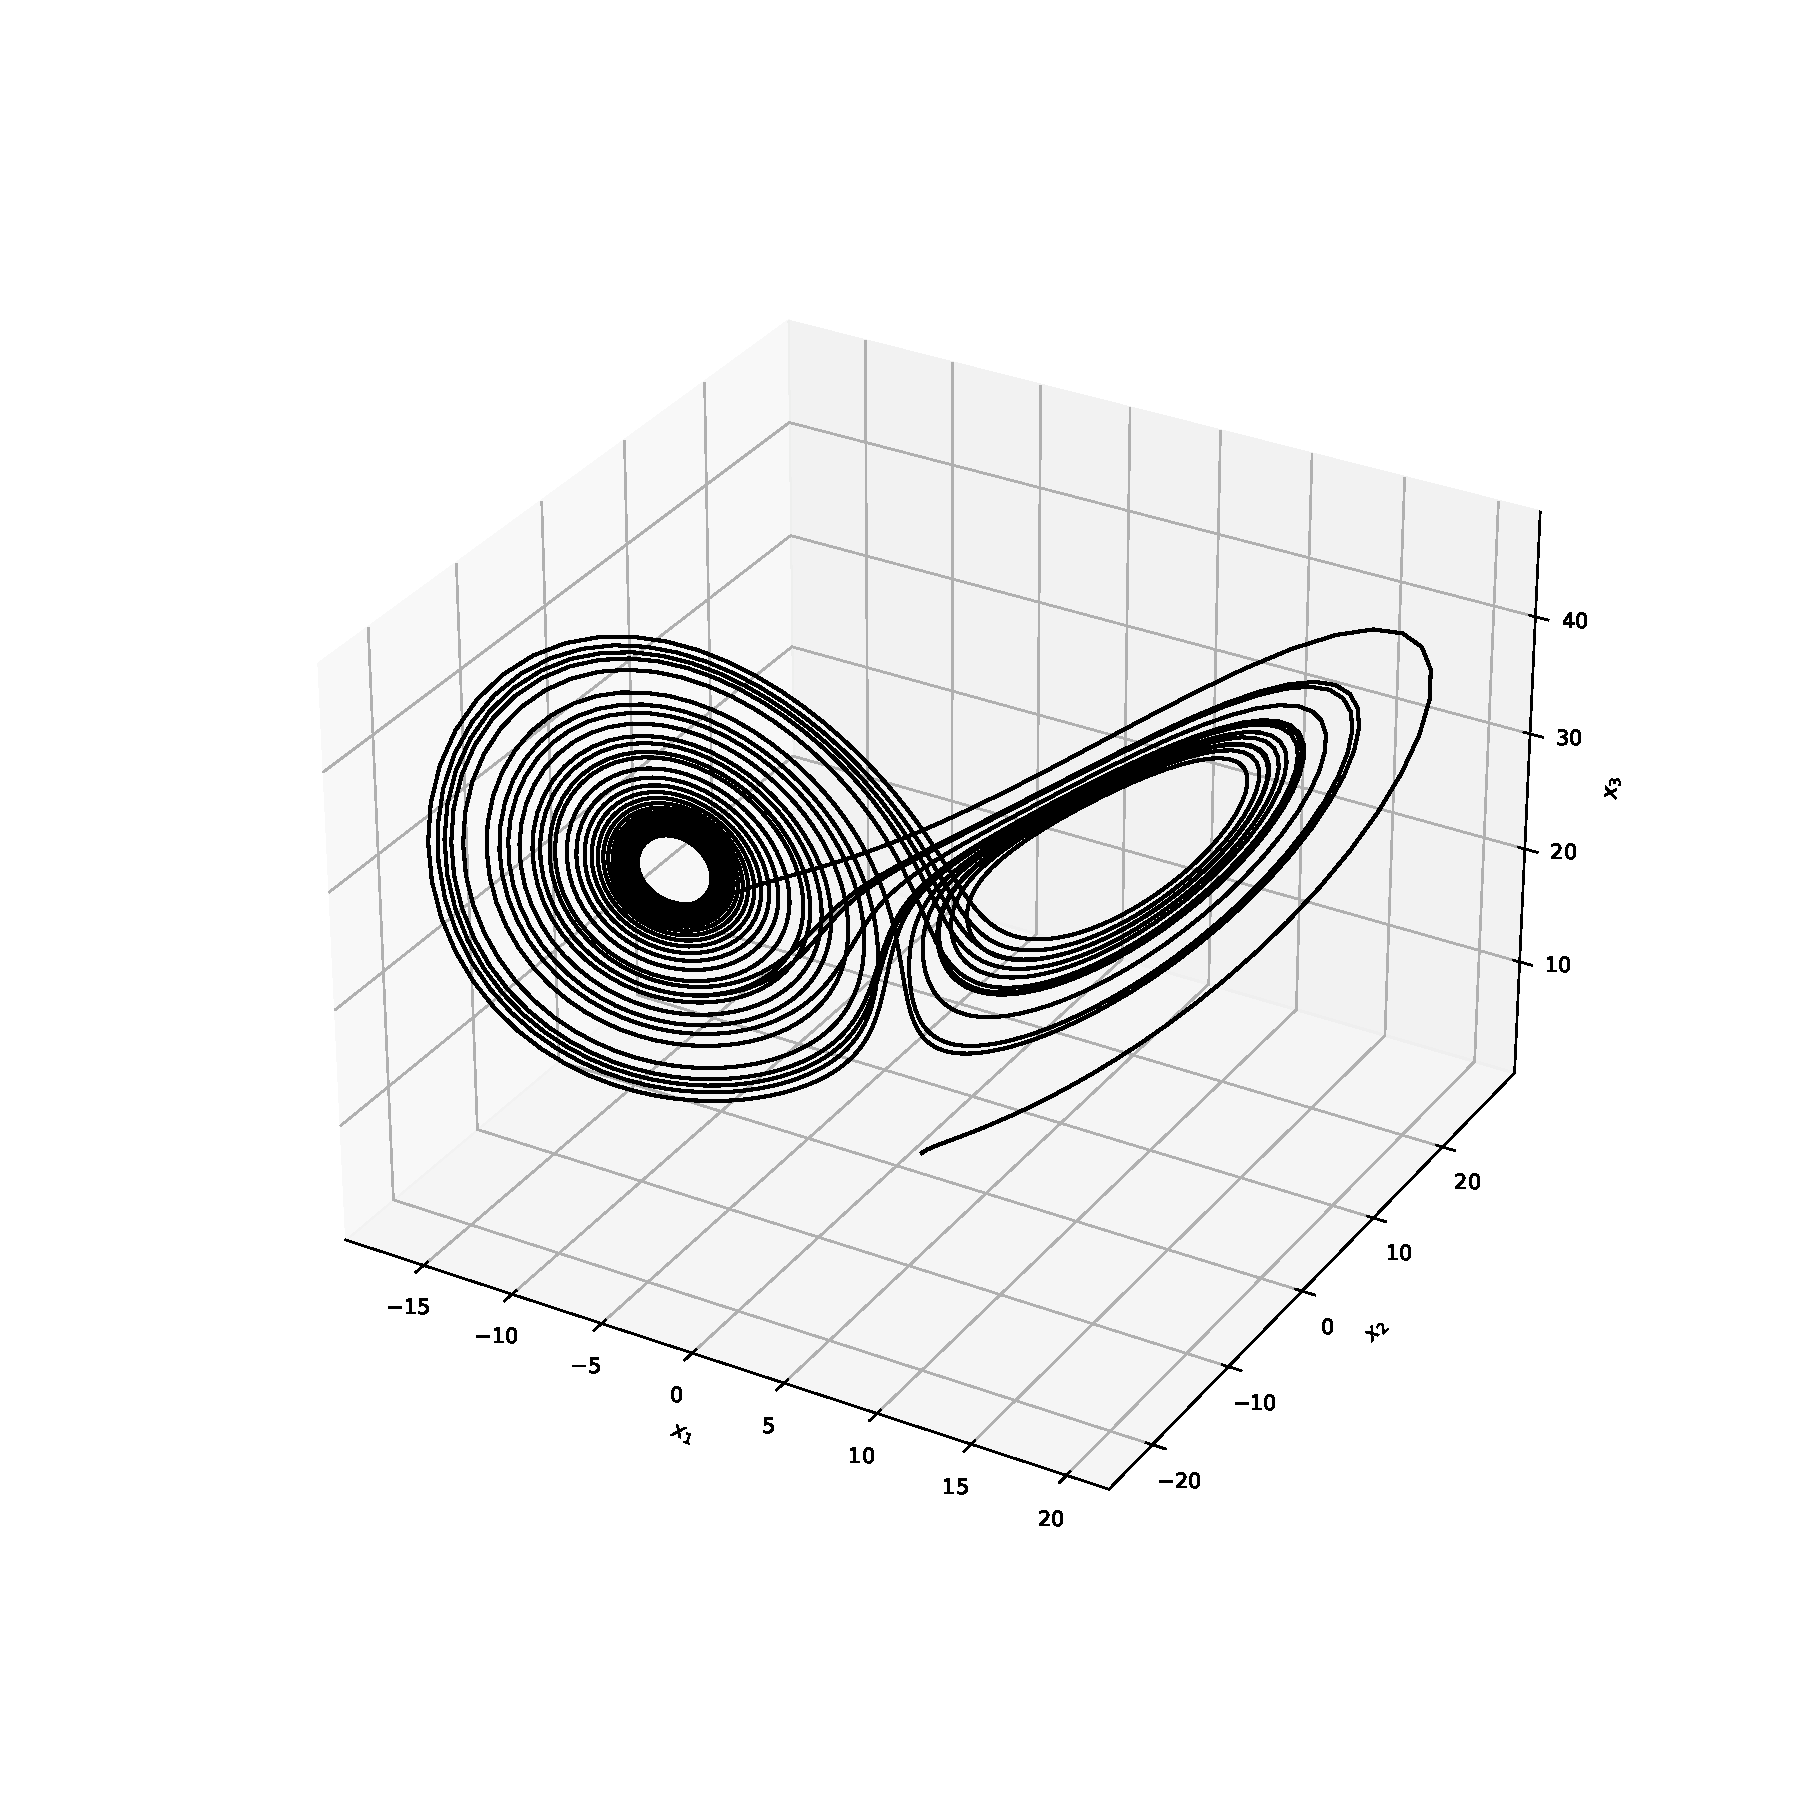
\includegraphics[trim=2cm 2cm 2cm 2cm, clip, scale=0.3]{Lorenz2.pdf}
  \caption{Initial condition $(0.999,1,1)$.}
  \label{subfig2:mp}
\end{subfigure}
\caption{Chaotic behavior of the Lorenz system with different initial conditions.}
\label{fig:LE}
\end{figure}   

In 1996, Dabby \cite{dabby_musical_1996} proposed a pioneering method for creating musical variations by exploiting the chaotic system \eqref{eq: lorenz}. 
This approach capitalizes on the sensitivity of chaotic trajectories to initial conditions and their long-term aperiodic dynamics, avoiding convergence towards equilibrium points. 
The method begins by establishing an injective mapping $g$ between a component of the numerical solution to the system \eqref{eq: lorenz} with an initial condition $x(0) \in \mathbb{R}^3$ and a sequence of musical pitches. 
Subsequently, a second chaotic trajectory of the system \eqref{eq: lorenz} is obtained by initializing it with a different initial condition $\tilde{x}(0)$ located in close proximity to $x(0)$. 
Finally, a new sequence of pitches is defined through an injective mapping related to the original mapping $g$, resulting in a variation of the original music.

\section{Main Result}
\label{sec: mainresult}
This section outlines the procedure for generating musical variations from a chaotic mapping and the incorporation of melodic variation with expanded rhythm. 
The first technique demonstrates how a chaotic mapping can be utilized to create new variations in musical pitch. 
Subsequently, the second technique combines the procedure of generating musical variations from a chaotic mapping with melodic variation involving expanded rhythm, thereby producing more intricate and captivating musical variations.

\subsection{Musical Variations from a Chaotic Mapping Method}
\label{ss: mvfacm}

This section presents an adaptation of the method proposed by Dabby \cite{dabby_musical_1996} for generating musical variations by exploiting chaotic dynamics.
Consider a sheet music with $m$ being a positive integer representing the number of notes, and $\displaystyle\{p_k\}_{k=0}^{m-1}$ being a sequence of musical pitches. Let
\begin{equation} \label{eq: odes}
\dot{x}(t) = f(t,x)
\end{equation}
define a chaotic dynamical system with an initial condition $x(0) \in \mathbb{R}^n$, where $f: \mathbb{R}_{+} \times \mathbb{R}^n \to \mathbb{R}^n$ is a continuous function.

Given a sequence $\{\phi_i(kh)\}_{k=0}^{m-1}$, where $\phi_i:\mathbb{R}_+ \to \mathbb{R}$ is a numerical solution in the $i$-th component of the system \eqref{eq: odes} for some $i \in \mathbb{N}_n$ and a step size $h$, we define a mapping $g$ as
\begin{equation} \label{eq: gmap}
g(\phi_i(kh)) := p_k
\end{equation}
for all $k \in \{0\}\cup\mathbb{N}_{m-1}$.

To generate a new variation of the music, we consider $\{\tilde{\phi}_i(kh)\}_{k=0}^{m-1}$ as a sequence of a new trajectory with the initial condition $\tilde{x}(0) \in \mathbb{R}^n$, where $\tilde{\phi}_i$ is a numerical solution in the $i$-th component to the system \eqref{eq: odes}, and $\tilde{x}(0)$ is located not far from $x(0)$, i.e., $\left\lVert x(0) - \tilde{x}(0) \right\rVert \leq d$ for some small positive number $d \in \mathbb{R}$.
We then define another mapping $l$ as:
\begin{equation} \label{eq: lmap}
l(\tilde{\phi}_i(kh)) :=
\begin{cases}
g(\phi_i(b)) & \text{if } \exists\; a, b \in \dom{\phi_i} \text{ s.t. } \phi_i(a) < \tilde{\phi}_i(kh) \leq \phi_i(b) \\
& \text{ and } \nexists\, c \in \dom{\phi_i} \text{ s.t. } \phi_i(a) < \phi_i(c) \leq \phi_i(b), \\
g(\phi_i(a)) & \text{if } \tilde{\phi}_i(kh) < \phi_i(a) \text{ for all } a \in \dom{\phi_i}, \\
g(\phi_i(b)) & \text{otherwise},
\end{cases}
\end{equation}
resulting in the sequence $\{l(\tilde{\phi}_i(kh))\}_{k=0}^{m-1}$, which represents a new variation of the original musical pitch.

\begin{example}
Consider the first three bars of the sheet music for the music ``Ah vous dirai-je Maman: \cite{hinson_12_1987}, illustrated in Figure \ref{fig:Dabby1}. 
The sequence
\[ \{p_k\}_{k=0}^{10} = \{C4, C4, G4, G4, A4, A4, G4, F4, F4, E4, E4\} \]
represents the pitches in this excerpt. 
Let 
\begin{equation} \label{eq: re}
\dot{x}(t) = f(t,x) = \begin{bmatrix}
 f_1(t, x) \\
 f_2(t, x) \\
 f_3(t, x) \\
\end{bmatrix}
:= 
\begin{bmatrix}
  10(x_2 - x_1) \\
  28x_1 - x_2 - x_1x_3 \\
  x_1x_2 - 2.6667x_3 \\
\end{bmatrix}
\end{equation} 
where $x = (x_1, x_2, x_3) \in \mathbb{R}^3$. 
Firstly, we consider the numerical solution in the first component to the system \eqref{eq: re} $\phi_1(t)$, derived using the fourth-order Runge-Kutta method with an initial condition $x(0) = (1,1,1)$ and a step size $h=0.01$.
The first eleven values of $\phi_1$ are represented by the sequence
 \[ \{ \phi_1(kh) \}_{k=0}^{10} = \{1.00, 1.29, 2.13, 3.74, 6.54, 11.04, 16.69, 19.56, 15.37, 7.55, 1.20\}. \]
We therefore define a mapping $g$ from $\{ \phi_1(kh) \}_{k=0}^{10}$ to $\{p_k\}_{k=0}^{10}$ according to the mapping \eqref{eq: gmap}, shown in Table \ref{table: gmap}.

Next, we consider the numerical solution in the first component to the system \eqref{eq: re} $\tilde{\phi}_1(t)$, derived again using the fourth-order Runge-Kutta method with the same step size, but with a different initial condition $\tilde{x}(0) = (1.01,1,1)$.
The first eleven values of $\tilde{\phi}_1$ is represented as
\[ \left\{\tilde{\phi}_1(kh) \right\}_{k=0}^{10} = \{ 1.01, 1.30, 2.15, 3.76, 6.58, 11.10, 16.73, 19.55, 15.30, 7.48, 1.15 \}. \] 
We then define a mapping $l$ from $\left\{\tilde{\phi}_1(kh) \right\}_{k=0}^{10}$ to new musical pitches according to the mapping \eqref{eq: lmap}, shown in Table \ref{table: lmap}.
This mapping $l$ produce the sequence \[ \{ l(\tilde{\phi}_1(kh)) \}_{k = 0}^{10} = \{E4, G4, G4, A4, E4, F4, F4, F4, F4, E4, E4 \}, \] illustrated in Figure \ref{fig:Dabby2}. 


The visualization of this method is illustrated in Figure \ref{fig:dabby method}. If we consider the musical notes that change at indices $k \in \{1, 2, 4, 5, 6, 7\}$, the change in pitch compared to the original musical pitches is approximately $54\%$. However, the audience might not distinguish the difference between the original and new notes as much as the change suggests, which makes this method less suitable for generating more interesting musical variations.

\begin{table}
\centering
\caption{The result of a mapping $g$ from $\{ \phi_1(kh) \}_{k=0}^{10}$ to $\{p_k\}_{k=0}^{10}$}
\begin{tabular}{|c||c|c|c|c|c|c|c|c|c|c|c|}
\hline
$k$ & 0 & 1 & 2 & 3 & 4 & 5 & 6 & 7 & 8 & 9 & 10 \\
\hline
$kh$ & 0 & 0.01 & 0.02 & 0.03 & 0.04 & 0.05 & 0.06 & 0.07 & 0.08 & 0.09 & 0.10 \\
\hline
$\phi_1(kh)$ & $1.00$ & $1.29$ & $2.13$ & $3.74$ & $6.54$ & $11.04$ & $16.69$ & $19.56$ & $15.37$ & $7.55$ & $1.20$ \\
\hline
$g(\phi_1(kh))$ & C4 & C4 & G4 & G4 & A4 & A4 & G4 & F4 & F4 & E4 & E4  \\
\hline
\end{tabular}
\label{table: gmap}
\end{table}

\begin{table}
\centering
\caption{The result of a mapping $l$ from $\left\{\tilde{\phi}_1(kh) \right\}_{k=0}^{10}$ to new musical pitches}
\begin{tabular}{|c||c|c|c|c|c|c|c|c|c|c|c|}
\hline
$k$ & 0 & 1 & 2 & 3 & 4 & 5 & 6 & 7 & 8 & 9 & 10 \\
\hline
$kh$ & 0 & 0.01 & 0.02 & 0.03 & 0.04 & 0.05 & 0.06 & 0.07 & 0.08 & 0.09 & 0.10 \\
\hline
$\tilde{\phi}_1(kh)$ & $1.01$ & $1.30$ & $2.15$ & $3.76$ & $6.58$ & $11.10$ & $16.73$ & $19.55$ & $15.30$ & $7.48$ & $1.15$ \\
\hline
$l(\tilde{\phi}_1(kh))$ & E4 & G4 & G4 & A4 & E4 & F4 & F4 & F4 & F4 & E4 & E4  \\
\hline
\end{tabular}
\label{table: lmap}
\end{table}

\end{example}

\begin{figure}
\centering
\begin{subfigure}{\textwidth}
  \centering
  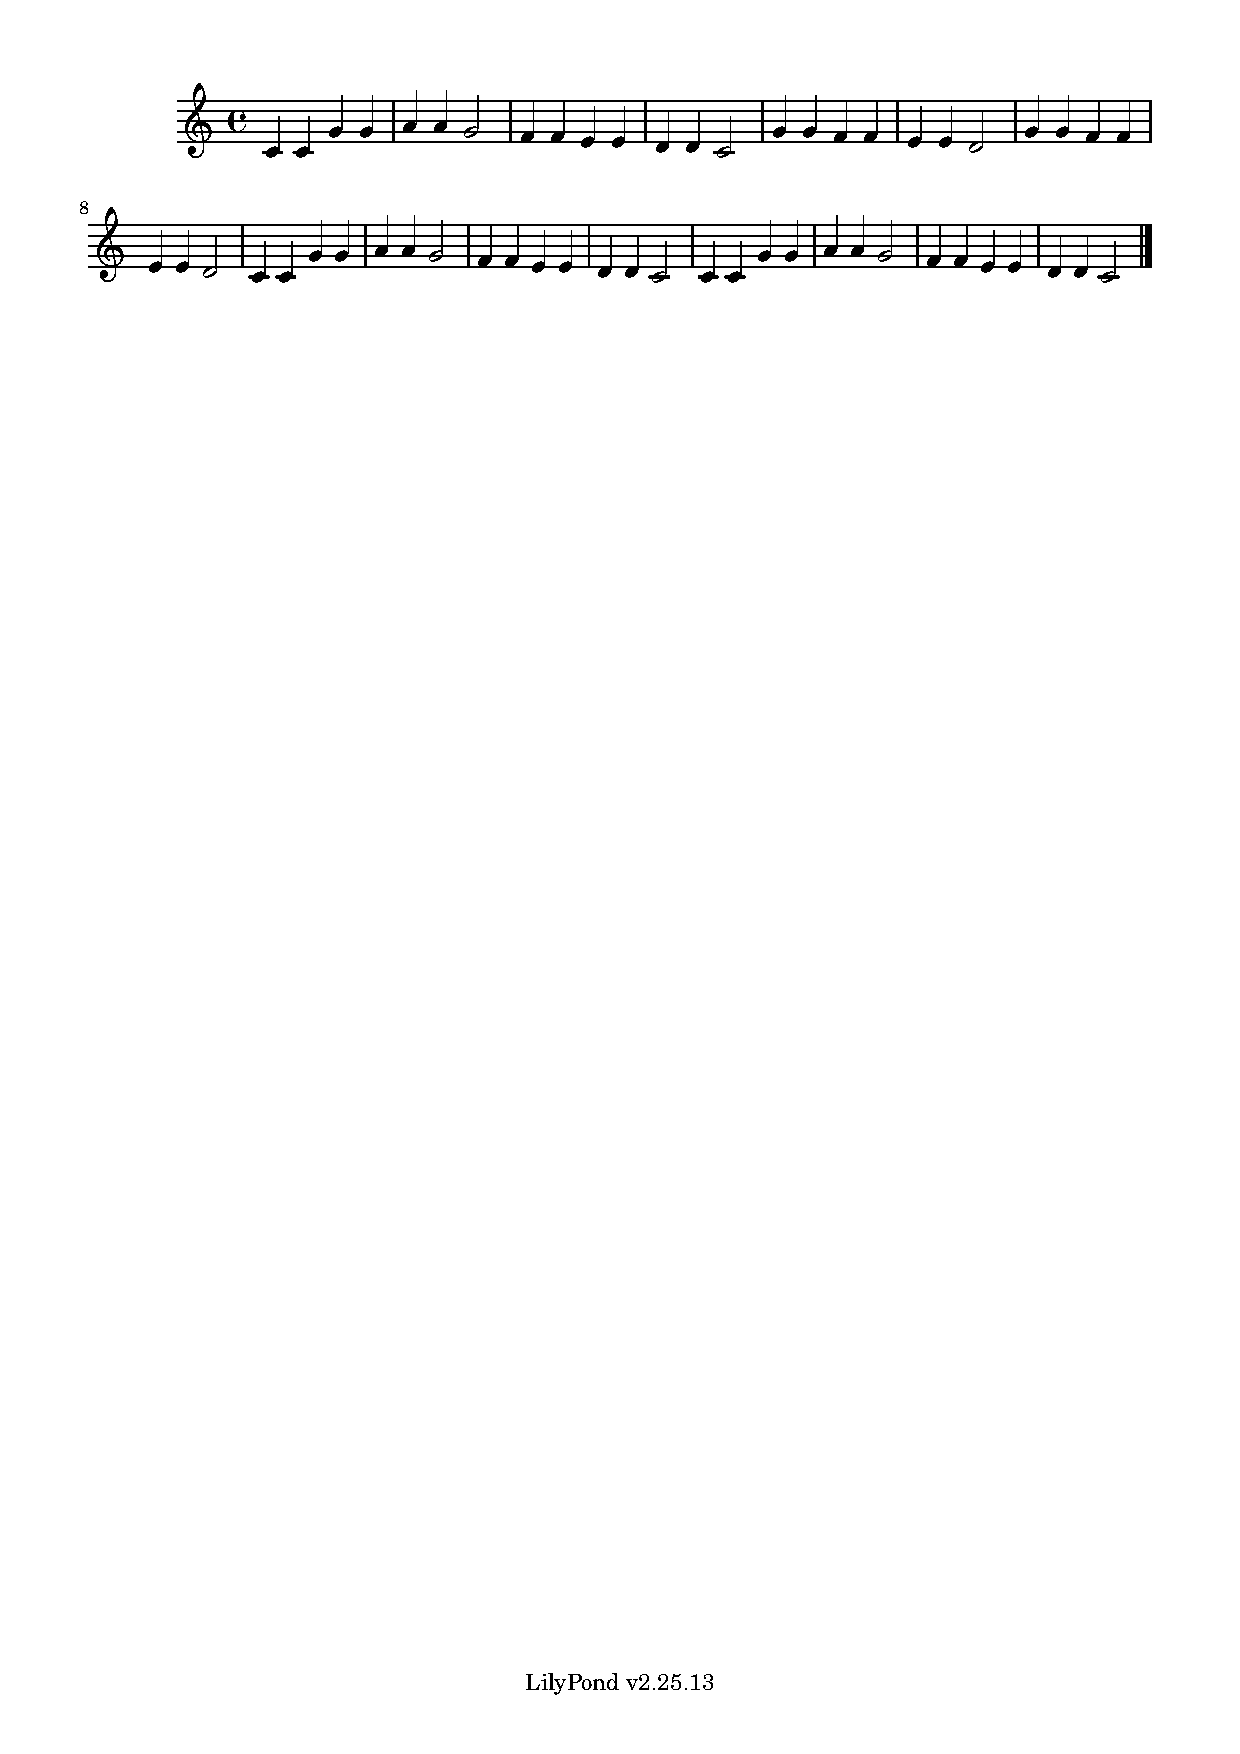
\includegraphics[trim=1cm 26.5cm 10.055cm 0.02cm, clip, scale=0.8]{dabby_1.pdf} % trim={left bottom right top}
  \caption{The original of Ah vous dirai-je Maman in the first 3 bars.}
  \label{fig:Dabby1} 
\end{subfigure}
\begin{subfigure}{\textwidth}
  \centering
  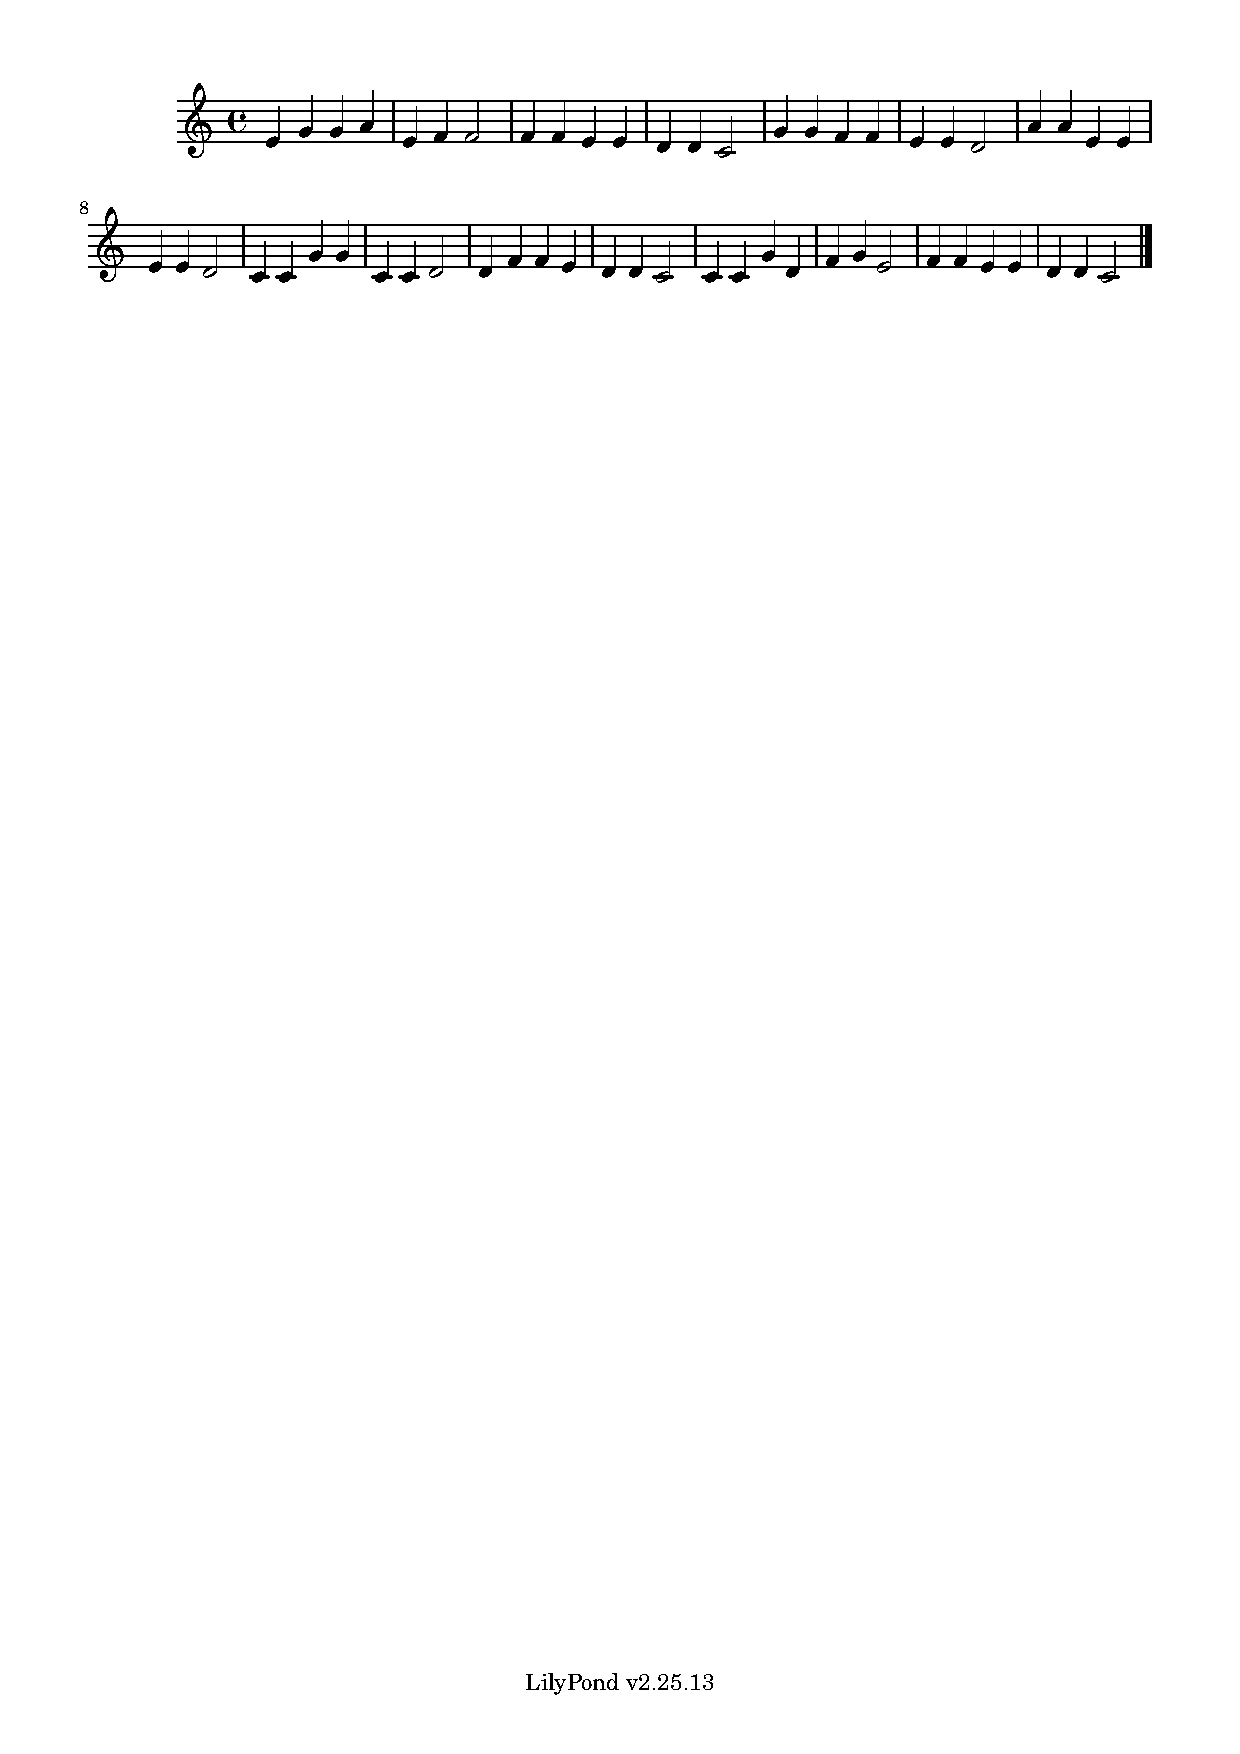
\includegraphics[trim=1cm 26.5cm 10.1cm 0.02cm, clip, scale=0.8]{dabby_2.pdf}
  \caption{The new variation of Ah vous dirai-je Maman in the first 3 bars, generated by the Initial Condition $(1.01, 1, 1)$.}
  \label{fig:Dabby2}
\end{subfigure}
\caption{The original and new variation of Ah vous dirai-je Maman}
\end{figure}

\begin{figure}
\centering

\begin{subfigure}{\textwidth}
  \centering
  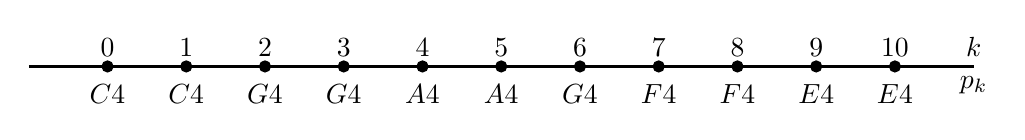
\begin{tikzpicture}
    % Draw number line
    \draw[-, thick] (0,0) -- (12,0) node[below] {$p_k$}  node[above] {$k$};

    % Data
    \foreach \i/\x/\p in {1/C4/0, 2/C4/1, 3/G4/2, 4/G4/3, 5/A4/4, 6/A4/5, 7/G4/6, 8/F4/7, 9/F4/8, 10/E4/9, 11/E4/10} {
      % Draw points and labels
      \filldraw (\i,0) circle (2pt) node[above] {$\p$};
      
      % Draw number scale below the line
      \draw (\i,-0.1) node[below] {$\x$};
    }

  \end{tikzpicture}
  \caption{The first 11 pitches of the Ah vous dirai-je Maman are marked below the 1D axis.}
  \label{subfig:mp}
\end{subfigure}

\vspace{5pt}

\begin{subfigure}{\textwidth}
  \centering
  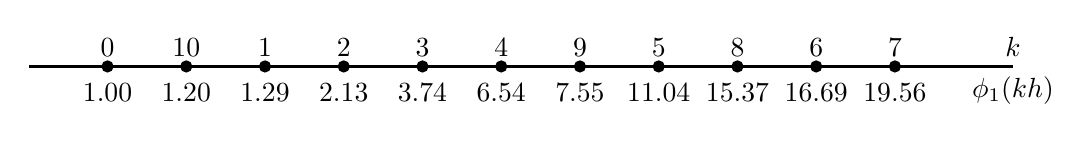
\begin{tikzpicture}
    % Draw number line
    \draw[-, thick] (0,0) -- (12.5,0) node[below] {$\phi_1(kh)$}  node[above] {$k$};

    % Data
    \foreach \i/\x/\p in {1/1.00/0, 2/1.20/10, 3/1.29/1, 4/2.13/2, 5/3.74/3, 6/6.54/4, 7/7.55/9, 8/11.04/5, 9/15.37/8, 10/16.69/6, 11/19.56/7} {
      % Draw points and labels
      \filldraw (\i,0) circle (2pt) node[above] {$\p$};
      
      % Draw number scale below the line
      \draw (\i,-0.1) node[below] {$\x$};
    }

  \end{tikzpicture}
  \caption{The first 11 numerical solution in first component to the system \eqref{eq: re} with initial condition of $(1,1,1)$ are marked below the 1D axis.}
  \label{subfig:traj1}
\end{subfigure}

\vspace{5pt}

\begin{subfigure}{\textwidth}
  \centering
  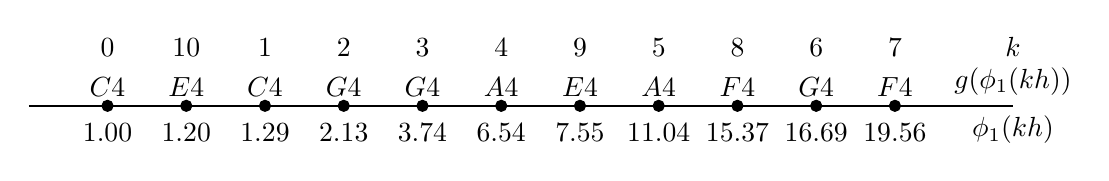
\begin{tikzpicture}
    % Draw number line
    \draw[-, thick] (0,0) -- (12.5,0) node[below] {$\phi_1(kh)$}  node[above] {$g(\phi_1(kh))$} node[above=0.5cm] {$k$};

    % Data
    \foreach \i/\x/\p in {1/1.00/C4, 2/1.20/E4, 3/1.29/C4, 4/2.13/G4, 5/3.74/G4, 6/6.54/A4, 7/7.55/E4, 8/11.04/A4, 9/15.37/F4, 10/16.69/G4, 11/19.56/F4} {
      % Draw points and labels
      \filldraw (\i,0) circle (2pt) node[above] {$\p$};
      
      % Draw number scale below the line
      \draw (\i,-0.1) node[below] {$\x$};
    }
    
    % Display the sequence at each point
    \foreach \i/\x in {1/0, 2/10, 3/1, 4/2, 5/3, 6/4, 7/9, 8/5, 9/8, 10/6, 11/7} {
      \draw (\i,0.5) node[above] {\x};
    }
  \end{tikzpicture}
  \caption{For each component in $\{\phi_1(kh)\}_{k=0}^{10}$, apply the $g(\phi_1(kh))$ mapping.}
  \label{subfig:traj1mp}

\end{subfigure}

\vspace{5pt}

\begin{subfigure}{\textwidth}
  \centering
  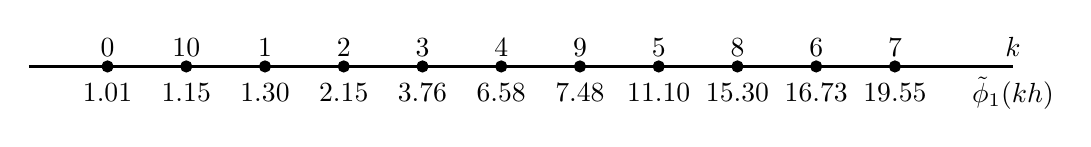
\begin{tikzpicture}
    % Draw number line
    \draw[-, thick] (0,0) -- (12.5,0) node[below] {$\tilde{\phi}_1(kh)$}  node[above] {$k$};

    % Data
    \foreach \i/\x/\p in {1/1.01/0, 2/1.15/10, 3/1.30/1, 4/2.15/2, 5/3.76/3, 6/6.58/4, 7/7.48/9, 8/11.10/5, 9/15.30/8, 10/16.73/6, 11/19.55/7} {
      % Draw points and labels
      \filldraw (\i,0) circle (2pt) node[above] {$\p$};
      
      % Draw number scale below the line
      \draw (\i,-0.1) node[below] {$\x$};
    }

  \end{tikzpicture}
  \caption{The first 11 numerical solution in first component to the system \eqref{eq: re} with new initial condition of $(1.01,1,1)$ are marked below the 1D axis.}
  \label{subfig:traj2}

\end{subfigure}

\vspace{5pt}

\begin{subfigure}{\textwidth}
  \centering
  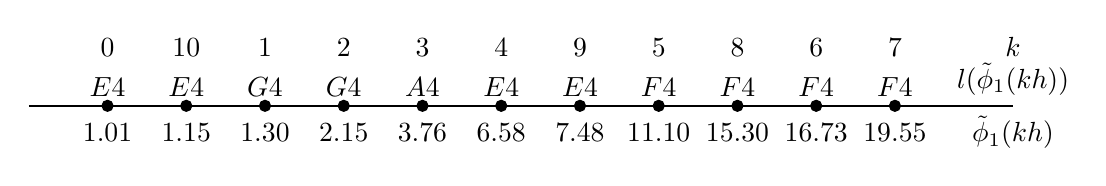
\begin{tikzpicture}
    % Draw number line
    \draw[-, thick] (0,0) -- (12.5,0) node[below] {$\tilde{\phi}_1(kh)$}  node[above] {$l(\tilde{\phi}_1(kh))$} node[above=0.5cm] {$k$};

    % Data
    \foreach \i/\x/\p in {1/1.01/E4, 2/1.15/E4, 3/1.30/G4, 4/2.15/G4, 5/3.76/A4, 6/6.58/E4, 7/7.48/E4, 8/11.10/F4, 9/15.30/F4, 10/16.73/F4, 11/19.55/F4} {
      % Draw points and labels
      \filldraw (\i,0) circle (2pt) node[above] {$\p$};
      
      % Draw number scale below the line
      \draw (\i,-0.1) node[below] {$\x$};
    }
    
    % Display the sequence at each point
    \foreach \i/\x in {1/0, 2/10, 3/1, 4/2, 5/3, 6/4, 7/9, 8/5, 9/8, 10/6, 11/7} {
      \draw (\i,0.5) node[above] {\x};
    }
  \end{tikzpicture}
  \caption{For each component in $\{\tilde{\phi}_1(kh)\}_{k=0}^{10}$, apply the $l(\tilde{\phi}_1(kh))$ mapping.}
  \label{subfig:traj2nmp}

\end{subfigure}

\vspace{5pt}

\begin{subfigure}{\textwidth}
  \centering
  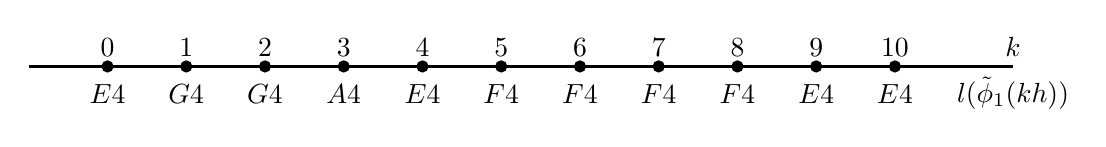
\begin{tikzpicture}
    % Draw number line
    \draw[-, thick] (0,0) -- (12.5,0) node[below] {$l(\tilde{\phi}_1(kh))$}  node[above] {$k$};

    % Data
    \foreach \i/\x/\p in {1/E4/0, 2/G4/1, 3/G4/2, 4/A4/3, 5/E4/4, 6/F4/5, 7/F4/6, 8/F4/7, 9/F4/8, 10/E4/9, 11/E4/10} {
      % Draw points and labels
      \filldraw (\i,0) circle (2pt) node[above] {$\p$};
      
      % Draw number scale below the line
      \draw (\i,-0.1) node[below] {$\x$};
    }
  \end{tikzpicture}
  \caption{The new variation of the first 11 pitches are marked below the 1D axis.}
  \label{subfig:nmp}

\end{subfigure}

\caption{The figure for visualizes how a chaotic mapping method can be used to generate musical variations}
\label{fig:dabby method}
\end{figure}

\subsection{Melodic Variation with Expanded Rhythm Method} 
\label{subsec: melodicvariationwithexpandedrhythm}

In this section, we present a technique for extending the rhythmic duration of musical notes, thereby opening up a number of possibilities for creating new musical variations. 
Let $\{p_k\}_{k=0}^{m-1}$ denote a sequence of music pitches. 
We can then establish a sequence of expanded music pitches $\{p^\prime_k\}_{k=0}^{mq-1}$, where $q$ is a positive integer representing the number of expanded notes for each $p_k$. Additionally, we set $p_k = p^\prime_{kq} = p^\prime_{kq + 1} = \dots = p^\prime_{q(k + 1) - 1}$.

\begin{example}
\label{ex: MV}
The sequence $ \{p_k\}_{k=0}^{3} = \{ C4, C4, G4, G4 \} $ represents the sequence of musical pitches in the first bar of the music piece ``Ah vous dirai-je Maman," as illustrated in Figure \ref{fig:MV1}.
Assuming $q = 4$ denotes the number of expanded notes for each $p_k$, we can establish an expanded sequence of musical pitches 
\[\{p^\prime_k\}_{k=0}^{15} = \{ C4, C4, C4, C4, C4, C4, C4, C4, G4, G4, G4, G4, G4, G4, G4, G4 \}, \] 
illustrated in Figure \ref{fig:MV2}.
\end{example}

\begin{figure}
\centering
\begin{subfigure}{\textwidth}
\centering
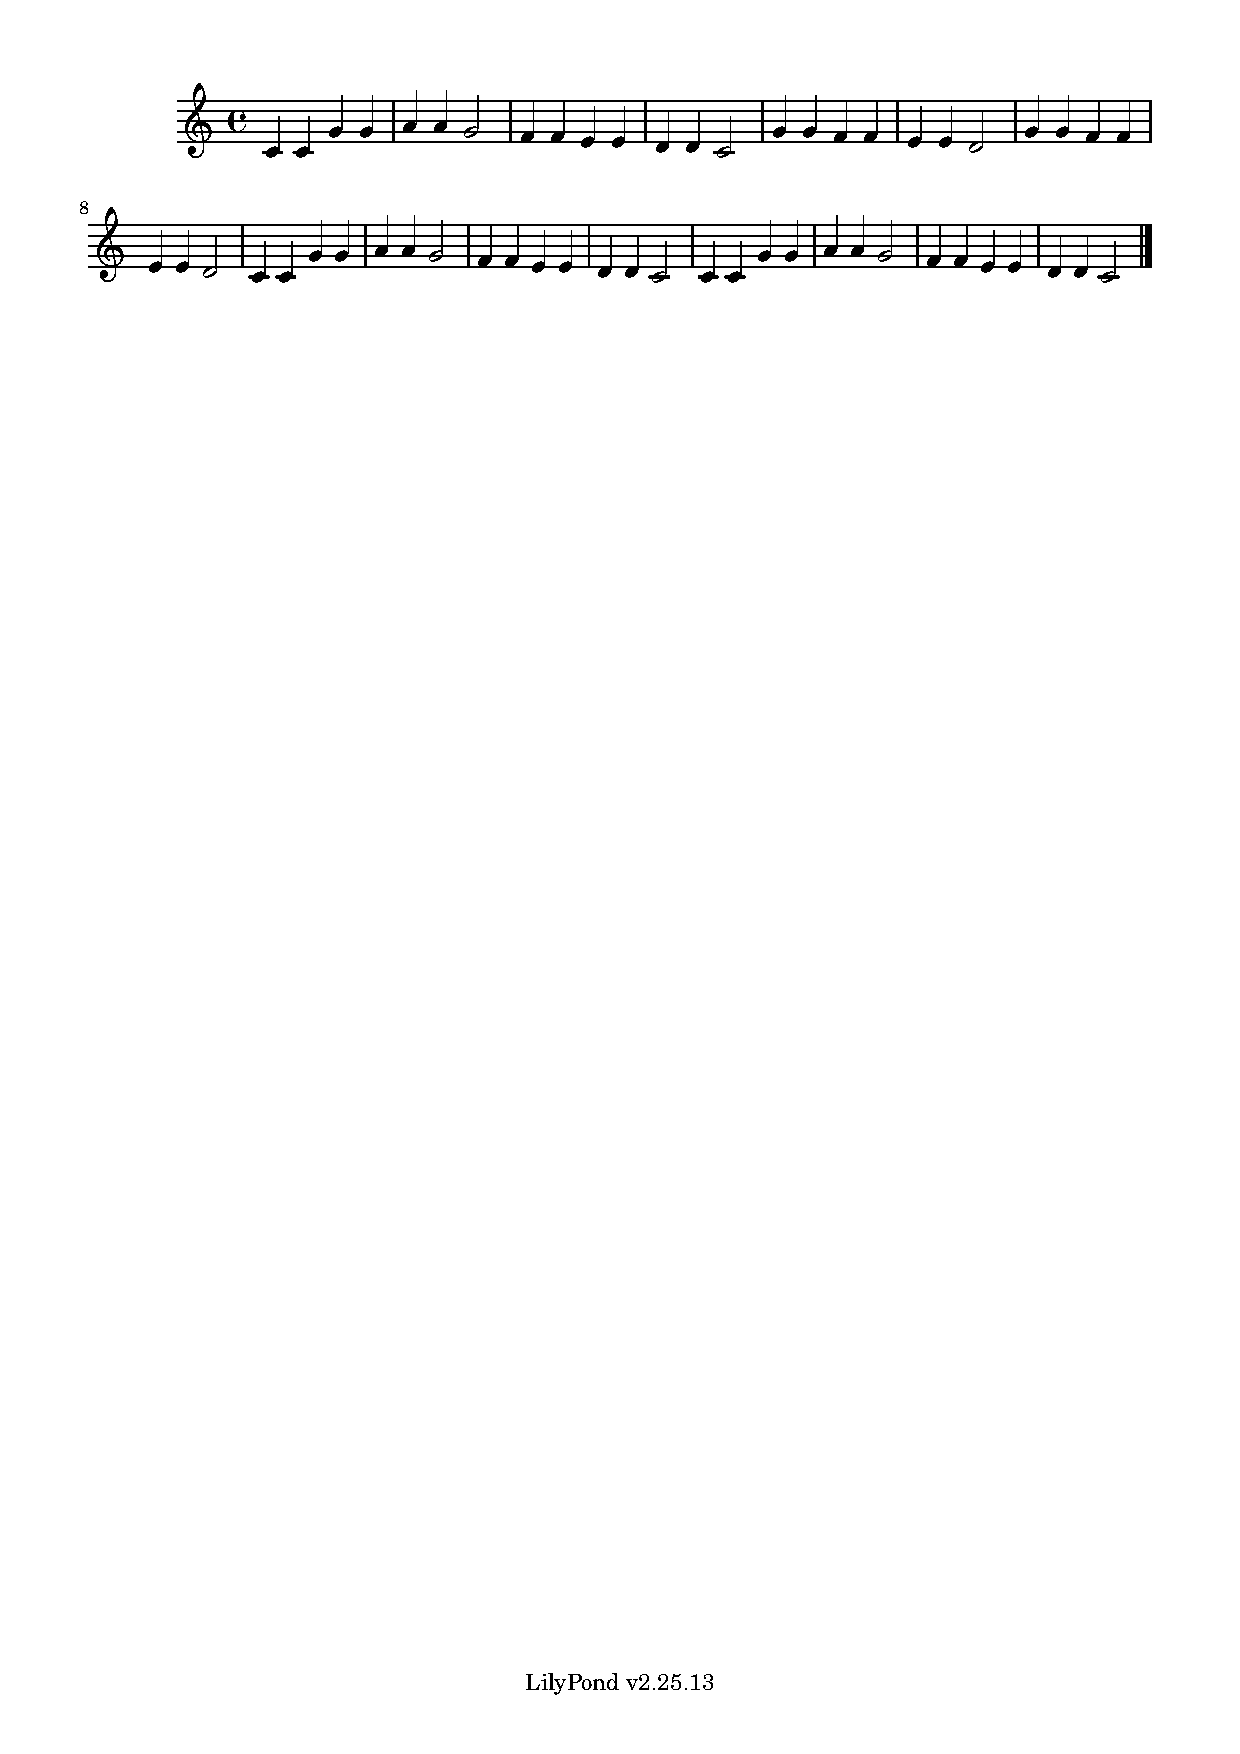
\includegraphics[trim=1cm 26.5cm 14.325cm 0.02cm, clip, scale=0.8]{dabby_1.pdf} % trim={left bottom right top}
\caption{The original of Ah vous dirai-je Maman in the first bars.}
\label{fig:MV1} 
\end{subfigure}
\begin{subfigure}{\textwidth}
\centering
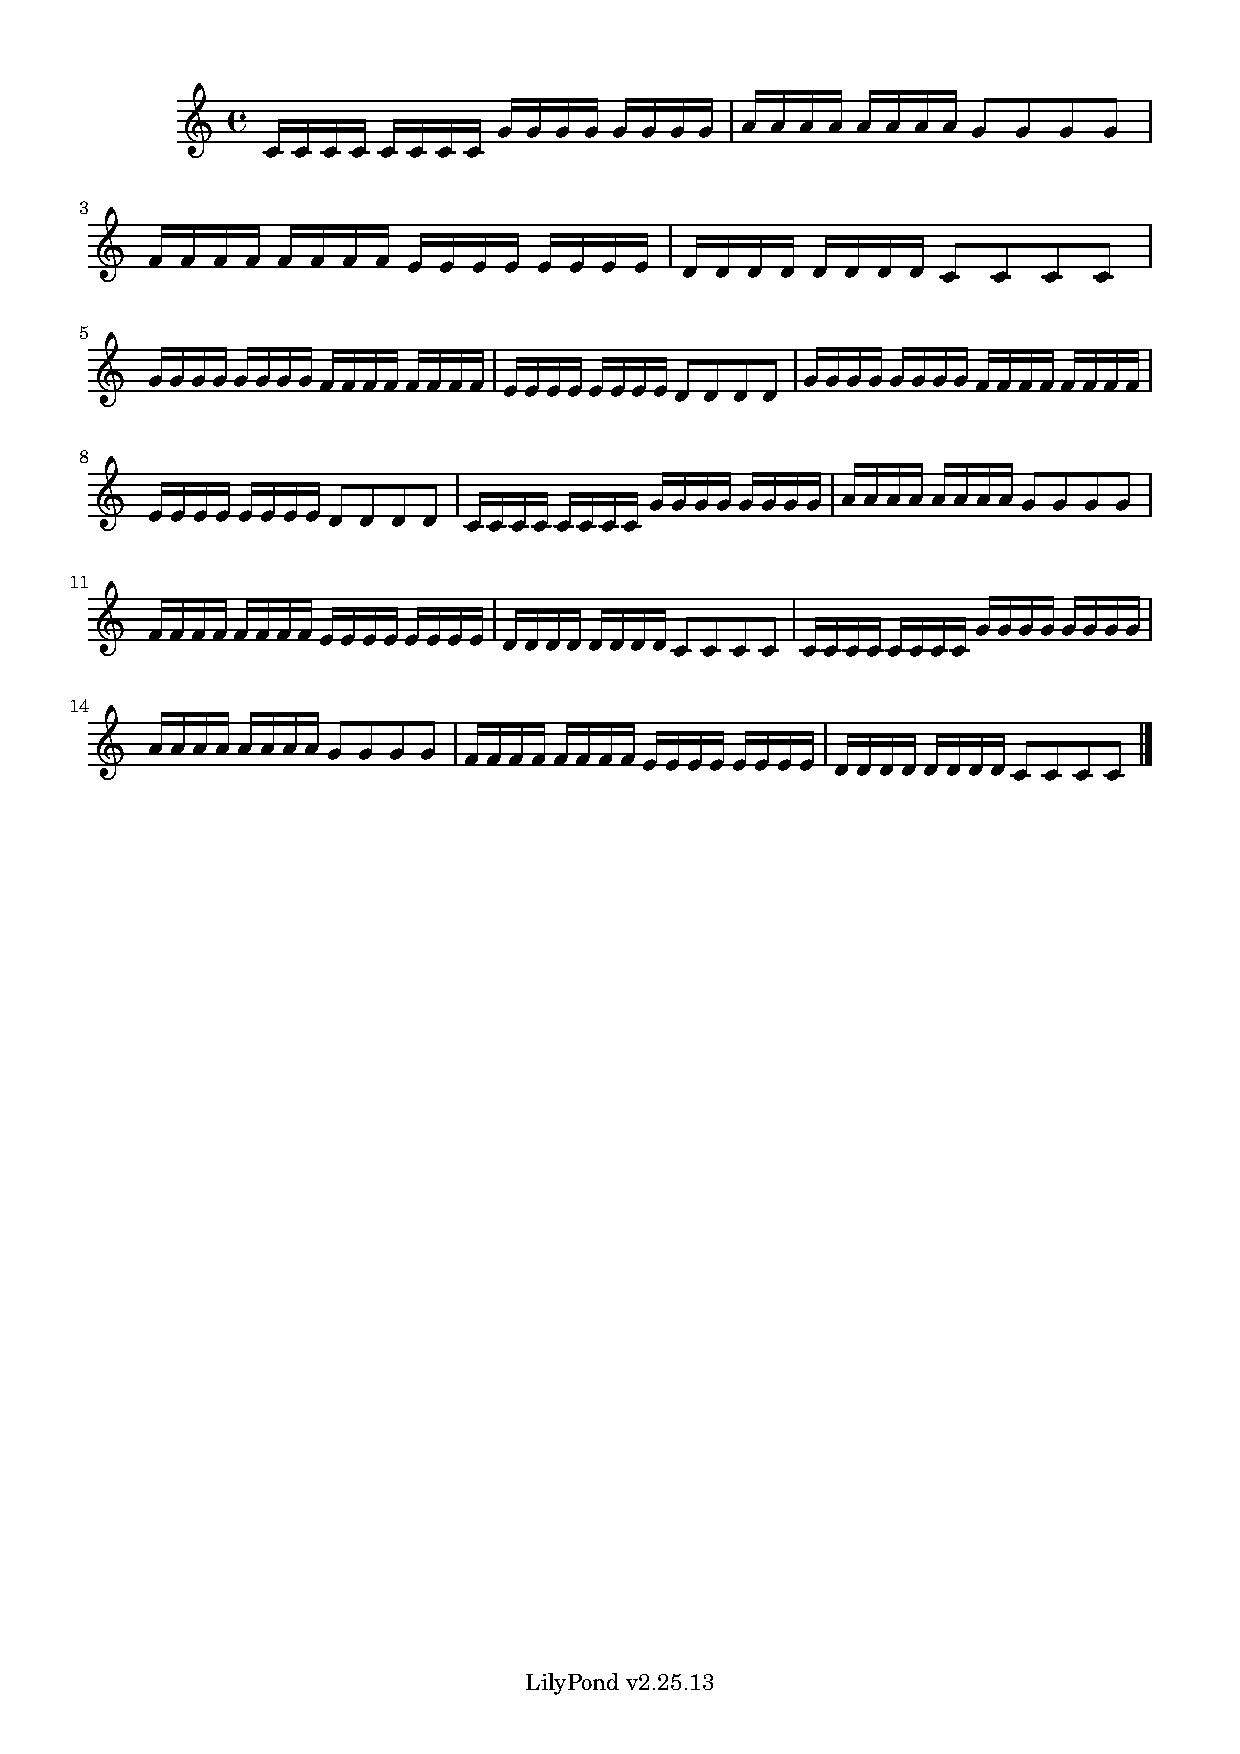
\includegraphics[trim=1cm 26.5cm 8.615cm 0.5cm, clip, scale=0.8]{melody_variation.pdf}
\caption{The melodic variation of Ah vous dirai-je, maman in the first bars.}
\label{fig:MV2}
\end{subfigure}
\caption{The original and melodic variation of Ah vous dirai-je Maman.}
\end{figure}

\begin{example}
Considering the sequence $\{p_k\}_{k=0}^{11}$ outlined in Example \ref{ss: mvfacm}, we proceed with the steps detailed in Section \ref{ss: mvfacm} to transition to the sequence $\{p^\prime_k\}_{k=0}^{15}$ as exemplified in Example \ref{ex: MV}. 
This transition utilizes the initial condition $x(0) = (0.5,0.5,0.5)$ and introduces a new trajectory initial condition $\tilde{x}(0) = (0.6,0.5,0.5)$.

Consequently, a sequence of new pitches is obtained:
\[ \{l(\tilde{\phi}_1(kh))\}_{k = 0}^{15} = \{C4, G4, D4, A4, A4, E4, F4, F4, F4, F4, E4, G4, D4, C4, C4, C4 \}, \]
which is depicted in Figure \ref{fig:DabbyER}. Furthermore, the visualization of this method is presented in Figure \ref{fig2:dabbymv method}. 
The resulting sequence of musical pitches exhibits significant divergence from the original sequence, with noticeable alterations in pitch that are perceivable by the audience. 
Such pronounced changes render this method conducive to generating more enchanting musical variations.
\end{example}

\begin{figure}
\centering
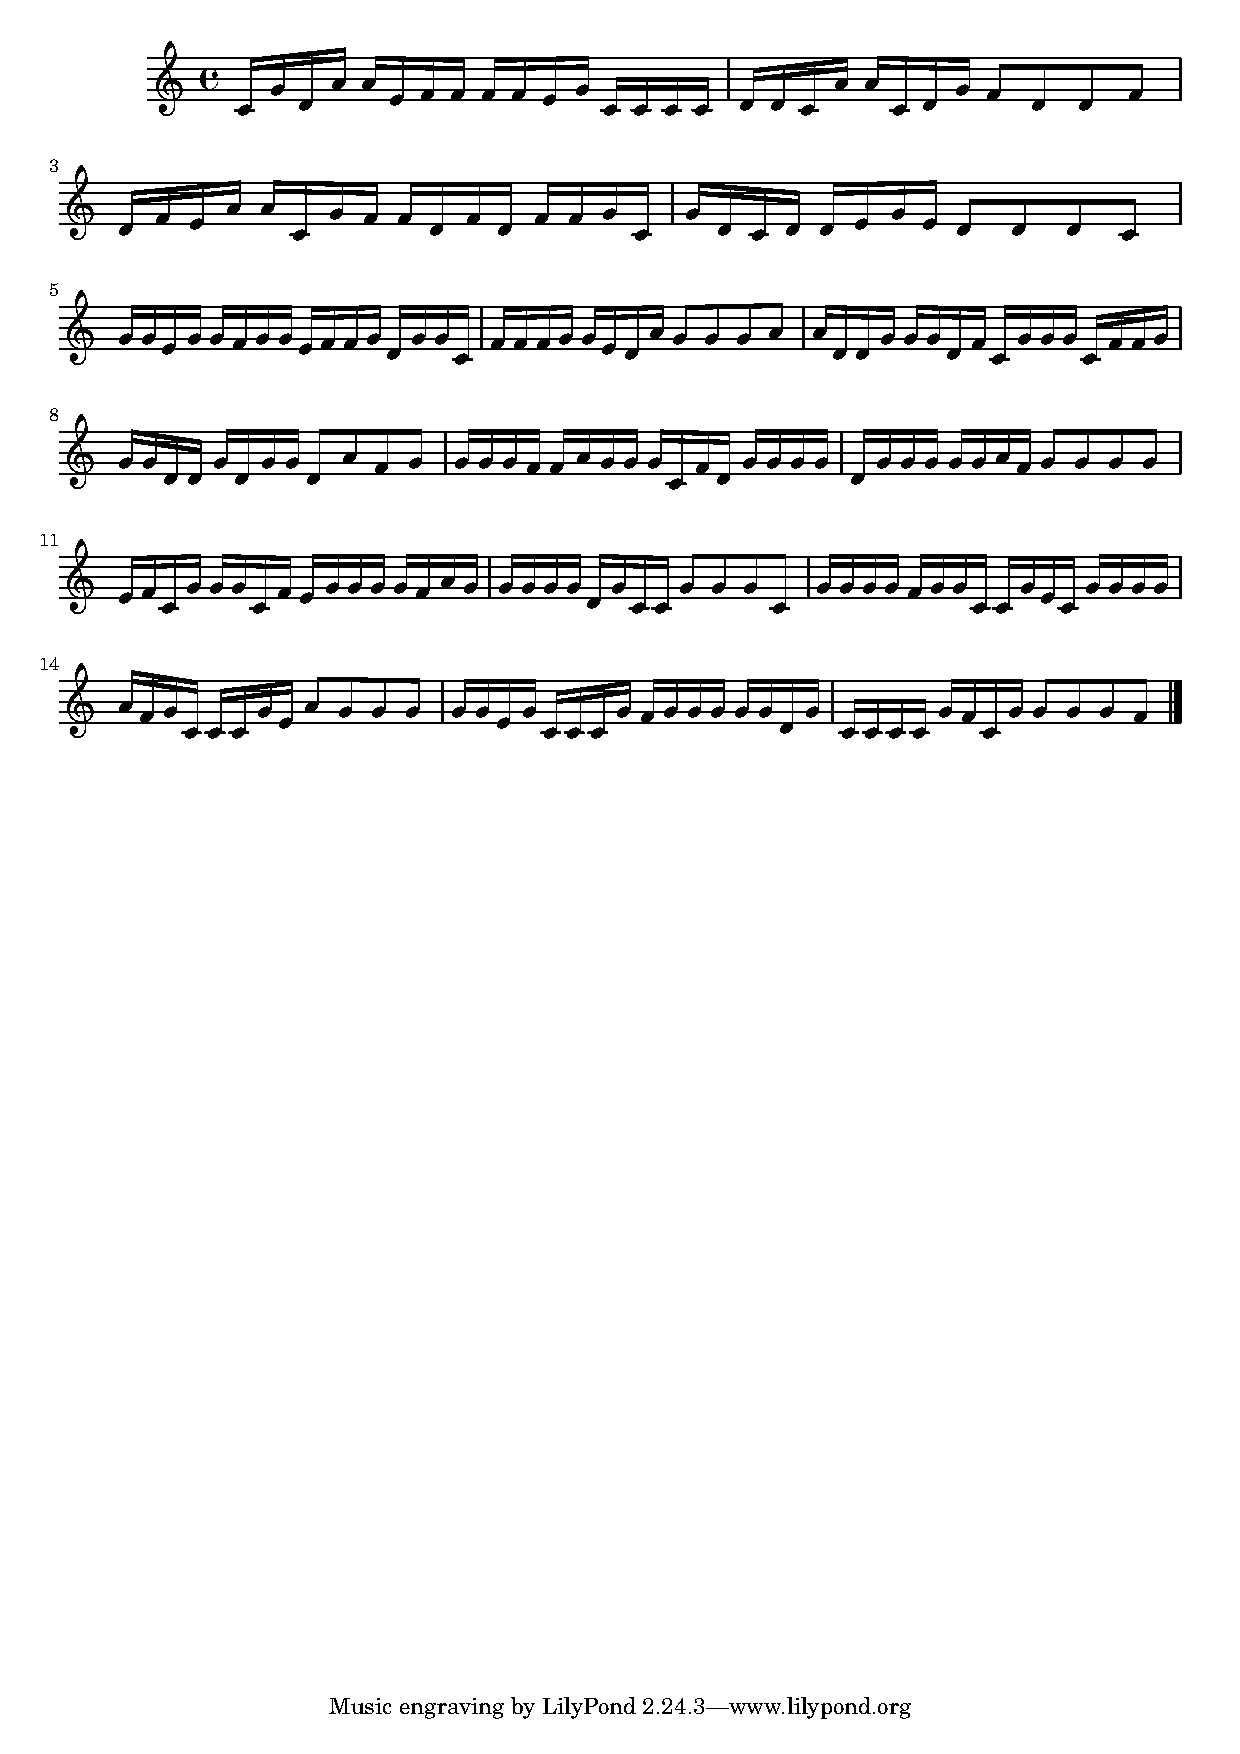
\includegraphics[trim=1cm 27.5cm 8.65cm 0.5cm, clip, scale=0.8]{dabby_melody_variation.pdf}
\caption{The new variation with melodic variation of Ah vous dirai-je, maman in the first bars, generated by the Initial Condition $(0.6, 0.5, 0.5)$.} 
\label{fig:DabbyER}
\end{figure}

\begin{figure}
\centering

\begin{subfigure}{\textwidth}
  \centering
  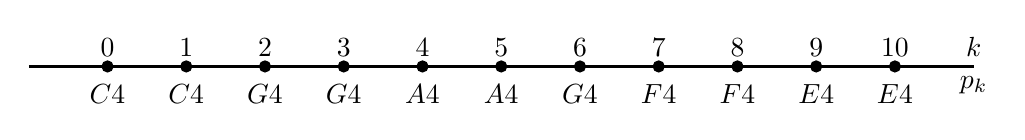
\begin{tikzpicture}
    % Draw number line
    \draw[-, thick] (0,0) -- (12,0) node[below] {$p_k$}  node[above] {$k$};

    % Data
    \foreach \i/\x/\p in {1/C4/0, 2/C4/1, 3/G4/2, 4/G4/3, 5/A4/4, 6/A4/5, 7/G4/6, 8/F4/7, 9/F4/8, 10/E4/9, 11/E4/10} {
      % Draw points and labels
      \filldraw (\i,0) circle (2pt) node[above] {$\p$};
      
      % Draw number scale below the line
      \draw (\i,-0.1) node[below] {$\x$};
    }

  \end{tikzpicture}
  \caption{The first 11 pitches of the Ah vous dirai-je Maman are marked below the 1D axis.}
  \label{subfig2:mp}
\end{subfigure}

\vspace{5pt}

\begin{subfigure}{\textwidth}
  \centering
  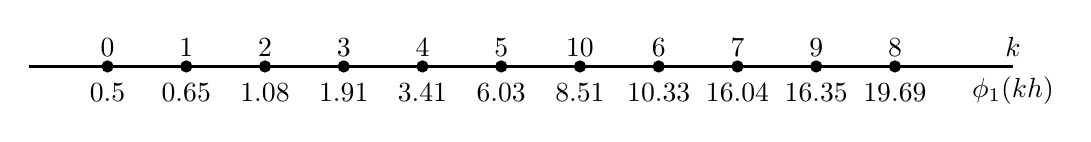
\begin{tikzpicture}
    % Draw number line
    \draw[-, thick] (0,0) -- (12.5,0) node[below] {$\phi_1(kh)$}  node[above] {$k$};

    % Data
    \foreach \i/\x/\p in {1/0.5/0, 2/0.65/1, 3/1.08/2, 4/1.91/3, 5/3.41/4, 6/6.03/5, 7/8.51/10, 8/10.33/6, 9/16.04/7, 10/16.35/9, 11/19.69/8} {
      % Draw points and labels
      \filldraw (\i,0) circle (2pt) node[above] {$\p$};
      
      % Draw number scale below the line
      \draw (\i,-0.1) node[below] {$\x$};
    }

  \end{tikzpicture}
  \caption{The first 11 numerical solution in first component to the system \eqref{eq: re} with initial condition of $(0.5,0.5,0.5)$ are marked below the 1D axis.}
  \label{subfig2:traj1}
\end{subfigure}

\vspace{5pt}

\begin{subfigure}{\textwidth}
  \centering
  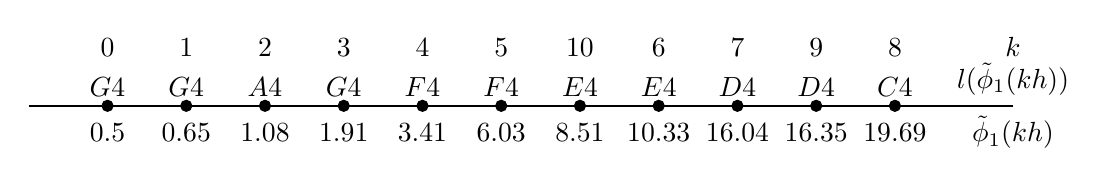
\begin{tikzpicture}
    % Draw number line
    \draw[-, thick] (0,0) -- (12.5,0) node[below] {$\tilde{\phi}_1(kh)$}  node[above] {$l(\tilde{\phi}_1(kh))$} node[above=0.5cm] {$k$};

    % Data
    \foreach \i/\x/\p in {1/0.5/G4, 2/0.65/G4, 3/1.08/A4, 4/1.91/G4, 5/3.41/F4, 6/6.03/F4, 7/8.51/E4, 8/10.33/E4, 9/16.04/D4, 10/16.35/D4, 11/19.69/C4} {
      % Draw points and labels
      \filldraw (\i,0) circle (2pt) node[above] {$\p$};
      
      % Draw number scale below the line
      \draw (\i,-0.1) node[below] {$\x$};
    }
    
    % Display the sequence at each point
    \foreach \i/\x in {1/0, 2/1, 3/2, 4/3, 5/4, 6/5, 7/10, 8/6, 9/7, 10/9, 11/8} {
      \draw (\i,0.5) node[above] {\x};
    }
  \end{tikzpicture}
  \caption{For each component in $\{\phi_1(kh)\}_{k=0}^{10}$, apply the $g(\phi_1(kh))$ mapping.}
  \label{subfig2:traj1mp}

\end{subfigure}

\vspace{5pt}

\begin{subfigure}{\textwidth}
  \centering
  \small{
  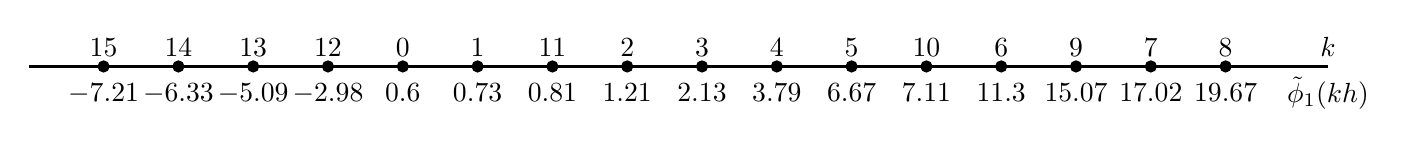
\begin{tikzpicture}
    % Draw number line
    \draw[-, thick] (0,0) -- (16.5,0) node[below] {$\tilde{\phi}_1(kh)$}  node[above] {$k$};

    % Data
    \foreach \i/\x/\p in {1/-7.21/15, 2/-6.33/14, 3/-5.09/13, 4/-2.98/12, 5/0.6/0, 6/0.73/1, 7/0.81/11, 8/1.21/2, 9/2.13/3, 10/3.79/4, 11/6.67/5, 12/7.11/10, 13/11.3/6, 14/15.07/9, 15/17.02/7, 16/19.67/8} {
      % Draw points and labels
      \filldraw (\i*0.95,0) circle (2pt) node[above] {$\p$};
      
      % Draw number scale below the line
      \draw (\i*0.95,-0.1) node[below] {$\x$};
    }

  \end{tikzpicture}}
  \caption{The first 16 numerical solution in first component to the system \eqref{eq: re} with new initial condition of $(0.6,0.5,0.5)$ are marked below the 1D axis.}
  \label{subfig2:traj2}

\end{subfigure}

\vspace{5pt}

\begin{subfigure}{\textwidth}
  \centering
  \small{
  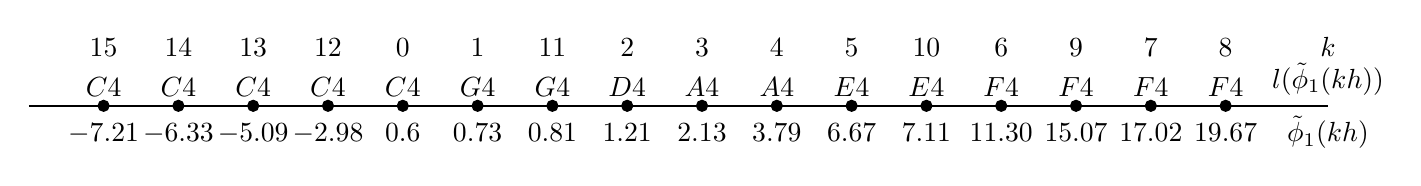
\begin{tikzpicture}
    % Draw number line
    \draw[-, thick] (0,0) -- (16.5,0) node[below] {$\tilde{\phi}_1(kh)$}  node[above] {$l(\tilde{\phi}_1(kh))$} node[above=0.5cm] {$k$};

    % Data
    \foreach \i/\x/\p in {1/-7.21/C4, 2/-6.33/C4, 3/-5.09/C4, 4/-2.98/C4, 5/0.6/C4, 6/0.73/G4, 7/0.81/G4, 8/1.21/D4, 9/2.13/A4, 10/3.79/A4, 11/6.67/E4, 12/7.11/E4, 13/11.30/F4, 14/15.07/F4, 15/17.02/F4, 16/19.67/F4} {
      % Draw points and labels
      \filldraw (\i*0.95,0) circle (2pt) node[above] {$\p$};
      
      % Draw number scale below the line
      \draw (\i*0.95,-0.1) node[below] {$\x$};
    }
    
    % Display the sequence at each point
    \foreach \i/\x in {1/15, 2/14, 3/13, 4/12, 5/0, 6/1, 7/11, 8/2, 9/3, 10/4, 11/5, 12/10, 13/6, 14/9, 15/7, 16/8} {
      \draw (\i*0.95,0.5) node[above] {\x};
    }
  \end{tikzpicture}}
  \caption{For each component in $\{\tilde{\phi}_1(kh)\}_{k=0}^{15}$, apply the $l(\tilde{\phi}_1(kh))$ mapping.}
  \label{subfig2:traj2nmp}

\end{subfigure}

\vspace{5pt}

\begin{subfigure}{\textwidth}
  \centering
  \small{
  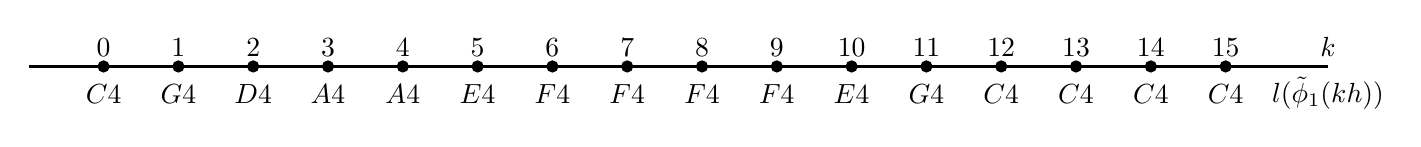
\begin{tikzpicture}
    % Draw number line
    \draw[-, thick] (0,0) -- (16.5,0) node[below] {$l(\tilde{\phi}_1(kh))$}  node[above] {$k$};

    % Data
    \foreach \i/\x/\p in {1/C4/0, 2/G4/1, 3/D4/2, 4/A4/3, 5/A4/4, 6/E4/5, 7/F4/6, 8/F4/7, 9/F4/8, 10/F4/9, 11/E4/10, 12/G4/11, 13/C4/12, 14/C4/13, 15/C4/14, 16/C4/15} {
      % Draw points and labels
      \filldraw (\i*0.95,0) circle (2pt) node[above] {$\p$};
      
      % Draw number scale below the line
      \draw (\i*0.95,-0.1) node[below] {$\x$};
    }

  \end{tikzpicture}}
  \caption{The new variation of the first 16 pitches are marked below the 1D axis.}
  \label{subfig2:nmp}

\end{subfigure}

\caption{The figure for visualizes how a chaotic mapping with melodic variation method can be used to generate musical variations}
\label{fig2:dabbymv method}
\end{figure}

\section{Discussion}
\label{sec: discussion}
This section explores the potential of combining musical variations from a chaotic mapping with melodic variation using an expanded rhythm method to generate diverse musical outcomes. Furthermore, we analyze the impact of this integrated approach on variations within other sheet music. For brevity, we'll refer to this combined methodology as the integrated approach. 

\subsection{Strengths of the Integrated Approach}

The integrated approach demonstrates promise in producing engaging musical variations, as evidenced by the new renditions featuring melodic variations of Pachelbel's Canon \cite{pachelbel_canon_2005} (Figure \ref{fig:NCND}), compared to the original melody (Figure \ref{fig:OCND}). 
Notably, this method proves particularly effective for compositions with a broad range of musical pitches. The expanded pitch range offers ample material for both chaotic mapping and melodic variation techniques, resulting in more intricate and varied musical outcomes.

This approach demonstrates enhanced effectiveness when applied to compositions featuring a broader range of musical pitches. The inclusion of additional pitches furnishes ample material for both chaotic mapping and melodic variation techniques to operate on, thereby yielding richer and more diverse musical variations.

\begin{figure}
\begin{subfigure}{\textwidth}
\centering
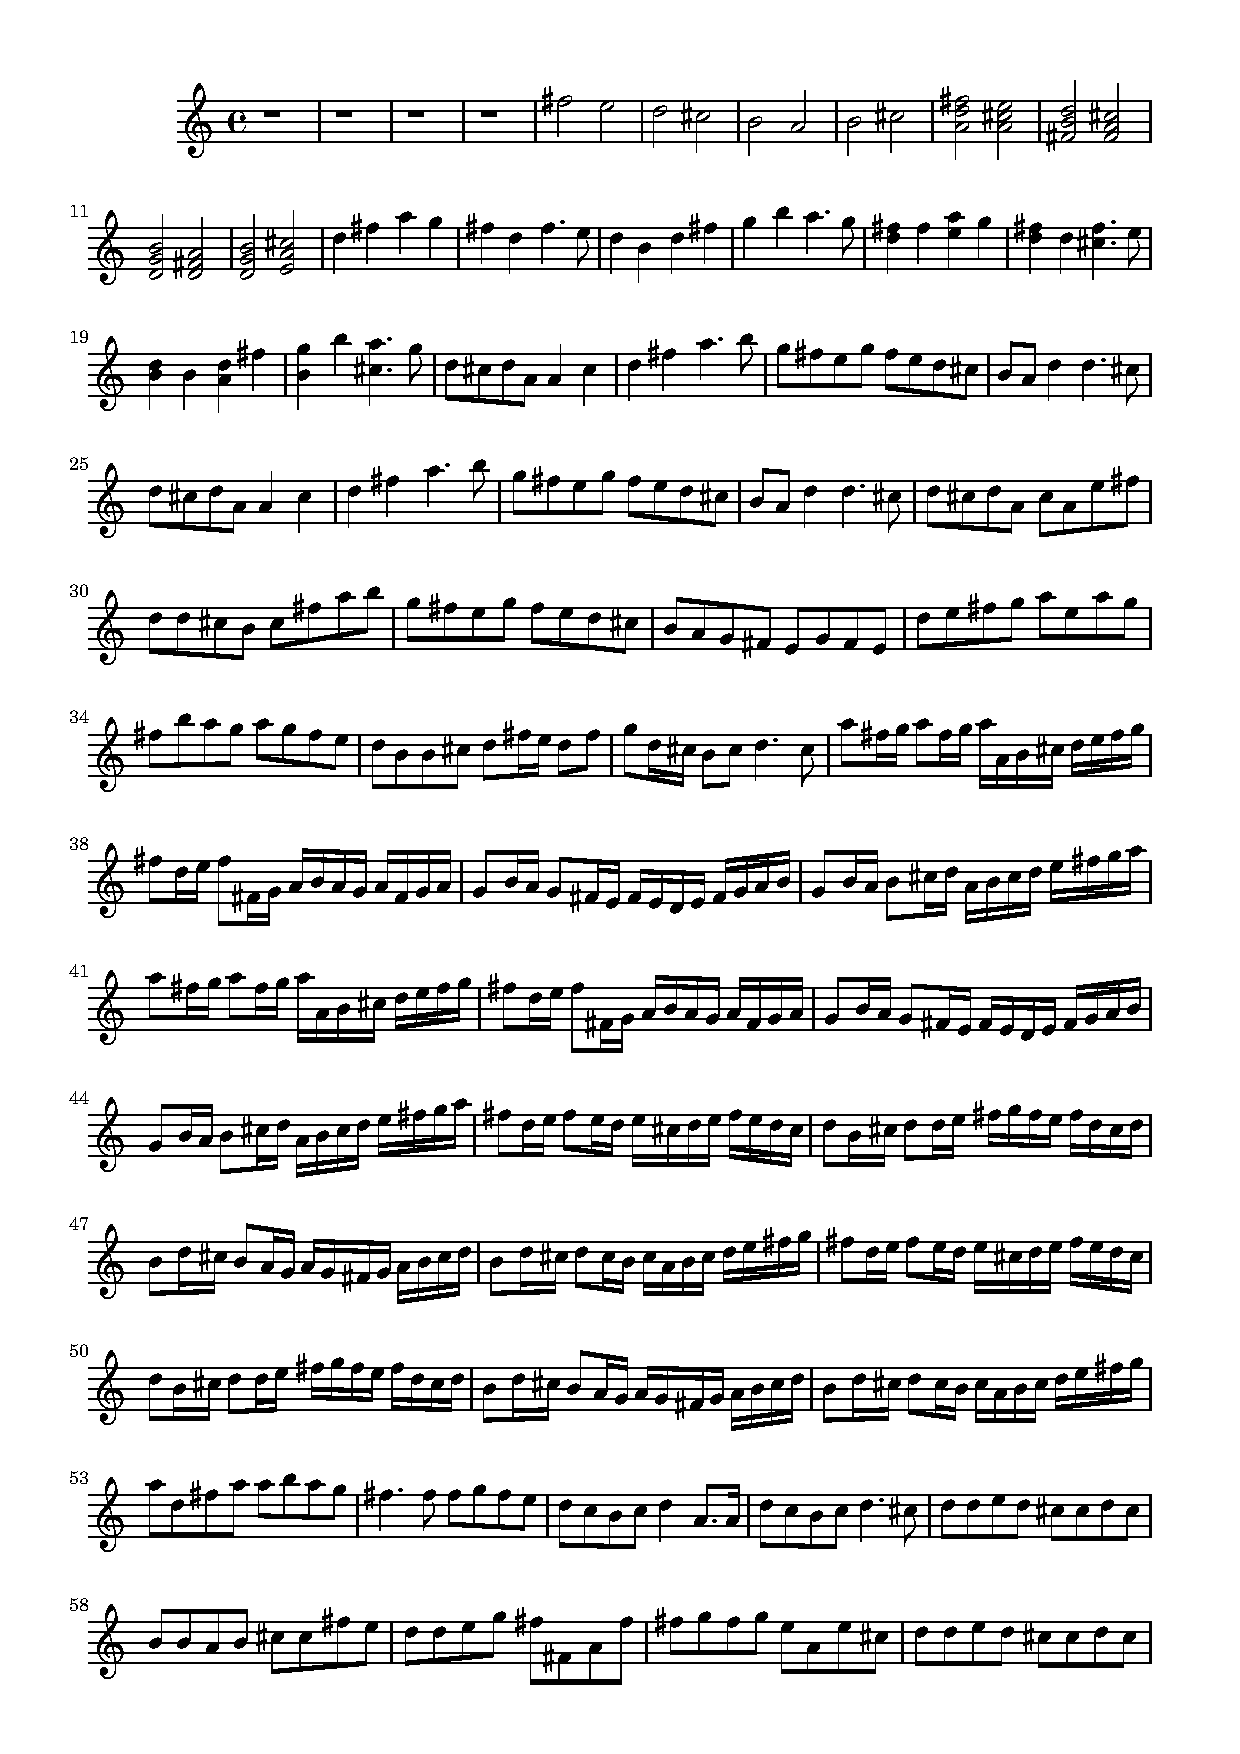
\includegraphics[trim=1cm 26.5cm 1cm 0.5cm, clip, scale=0.8]{Original_CND.pdf}
\caption{The original of Pachelbel's Canon in the first 10 bars.} 
\label{fig:OCND}
\end{subfigure}
\begin{subfigure}{\textwidth}
\centering
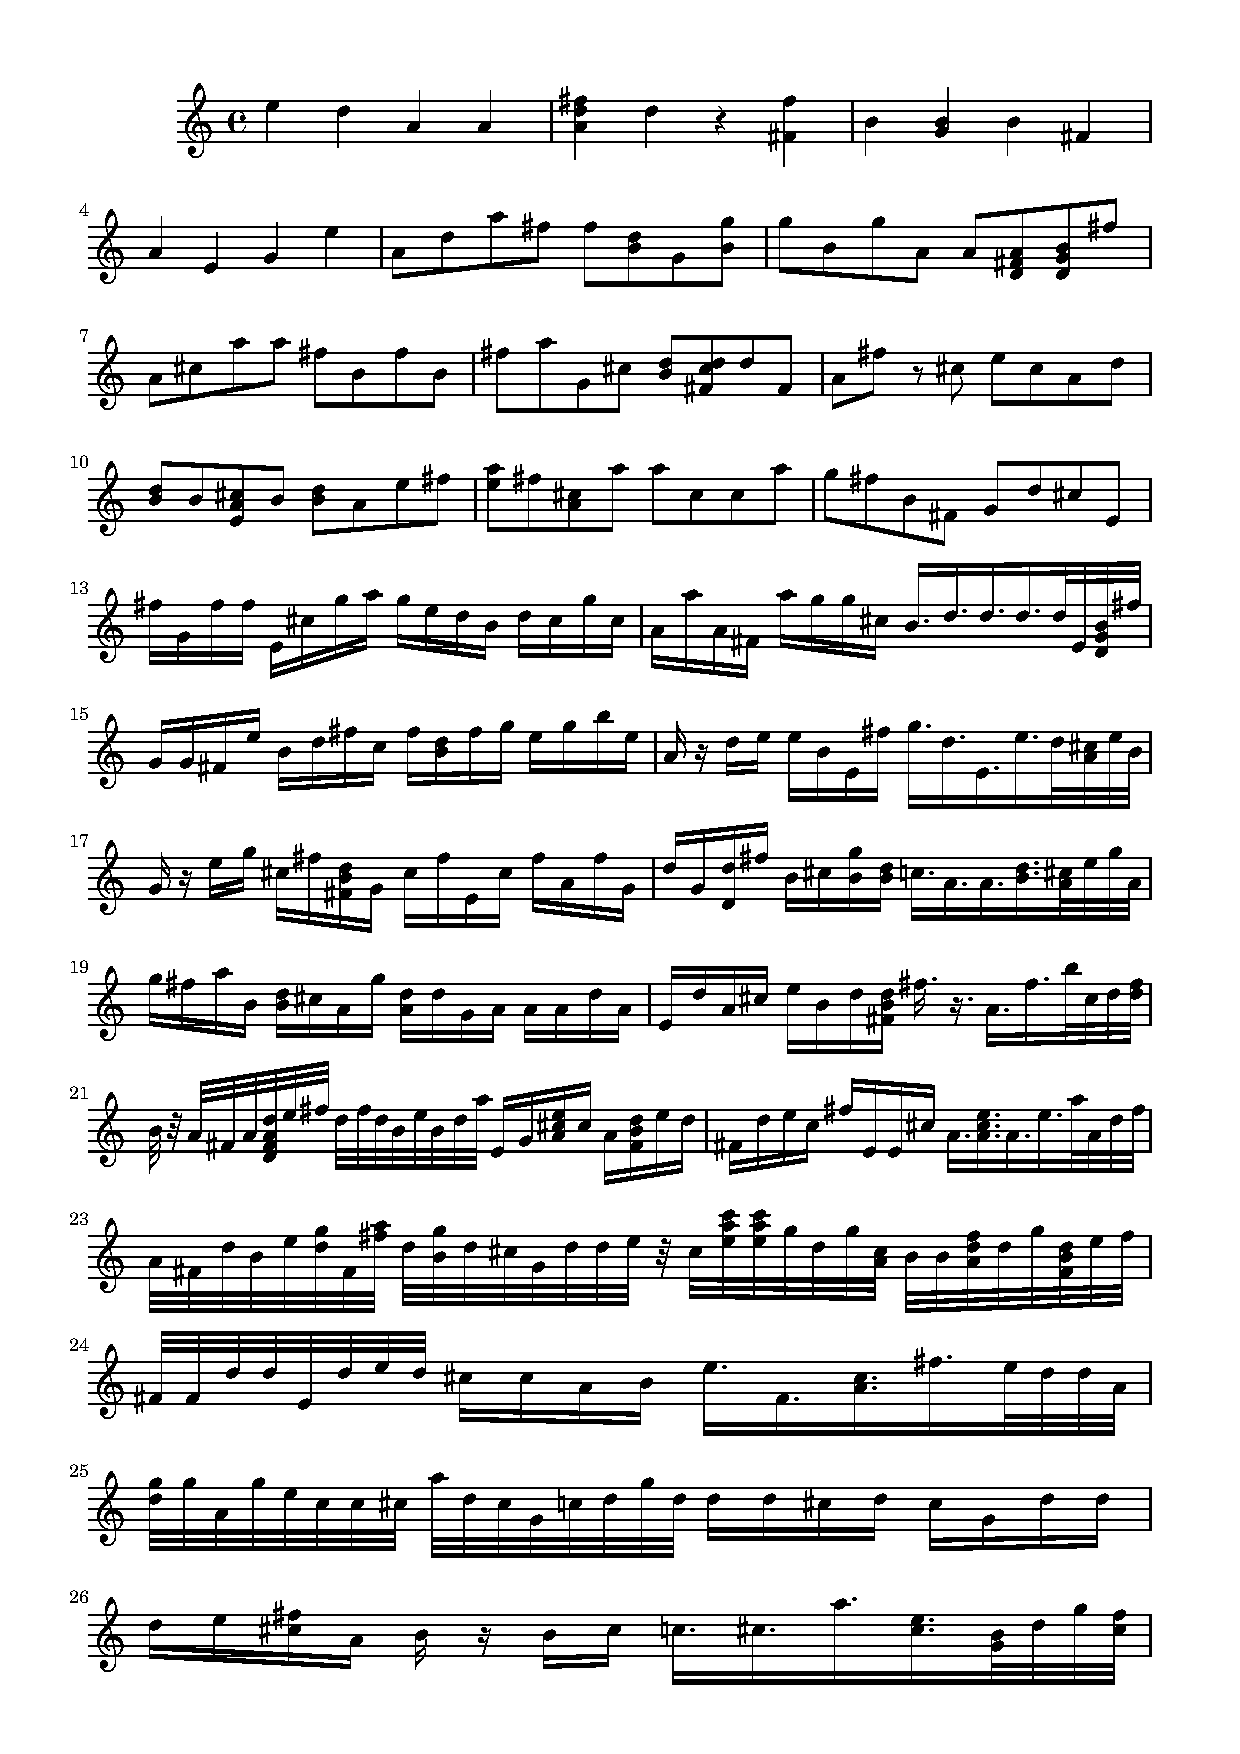
\includegraphics[trim=1cm 20.3cm 1cm 0.5cm, clip, scale=0.8]{New_CND.pdf}
\caption{The new variation with melodic variation of Pachelbel's Canon in the first 10 bars (including 2 additional bars at the end of the 10th bar).} 
\label{fig:NCND}
\end{subfigure}
\caption{The combined approach with Pachelbel's Canon in the first 10 bars.} 
\label{fig: exam1}
\end{figure}

\subsection{Weaknesses of the Integrated Approach}

Let us consider the sheet music for ``A Thousand Miles" \cite{carlton2009thousandmiles}, illustrated in Figure \ref{fig:OATM}, alongside a new variation produced through melodic manipulation, illustrated in Figure \ref{fig:NATM}. 
This comparison underscores a significant limitation of the method: when applied to compositions featuring a multitude of musical note durations, it may yield variations with melodies that prove challenging both to execute and to perceive.

The complexity inherent in compositions with varied note durations can pose difficulties for the integrated method, resulting in melodies that may be intricate to play and demanding to appreciate audibly. 
This observation emphasizes a notable weakness in the integrated approach, particularly when confronted with compositions characterized by a high degree of rhythmic complexity.

Additional assessment across a diverse array of musical compositions is imperative to establish the broader applicability of these findings. 
The advantage of the integrated approach may differ dependent upon the specific musical genre and attributes inherent in the original piece. 
Moreover, it is essential to consider the computational complexity associated with the chaotic mapping technique. 
While it presents a potential direction for music variation, it may necessitate heightened processing capabilities in comparison to simpler melodic variation methods.

\begin{figure}
\begin{subfigure}{\textwidth}
\centering
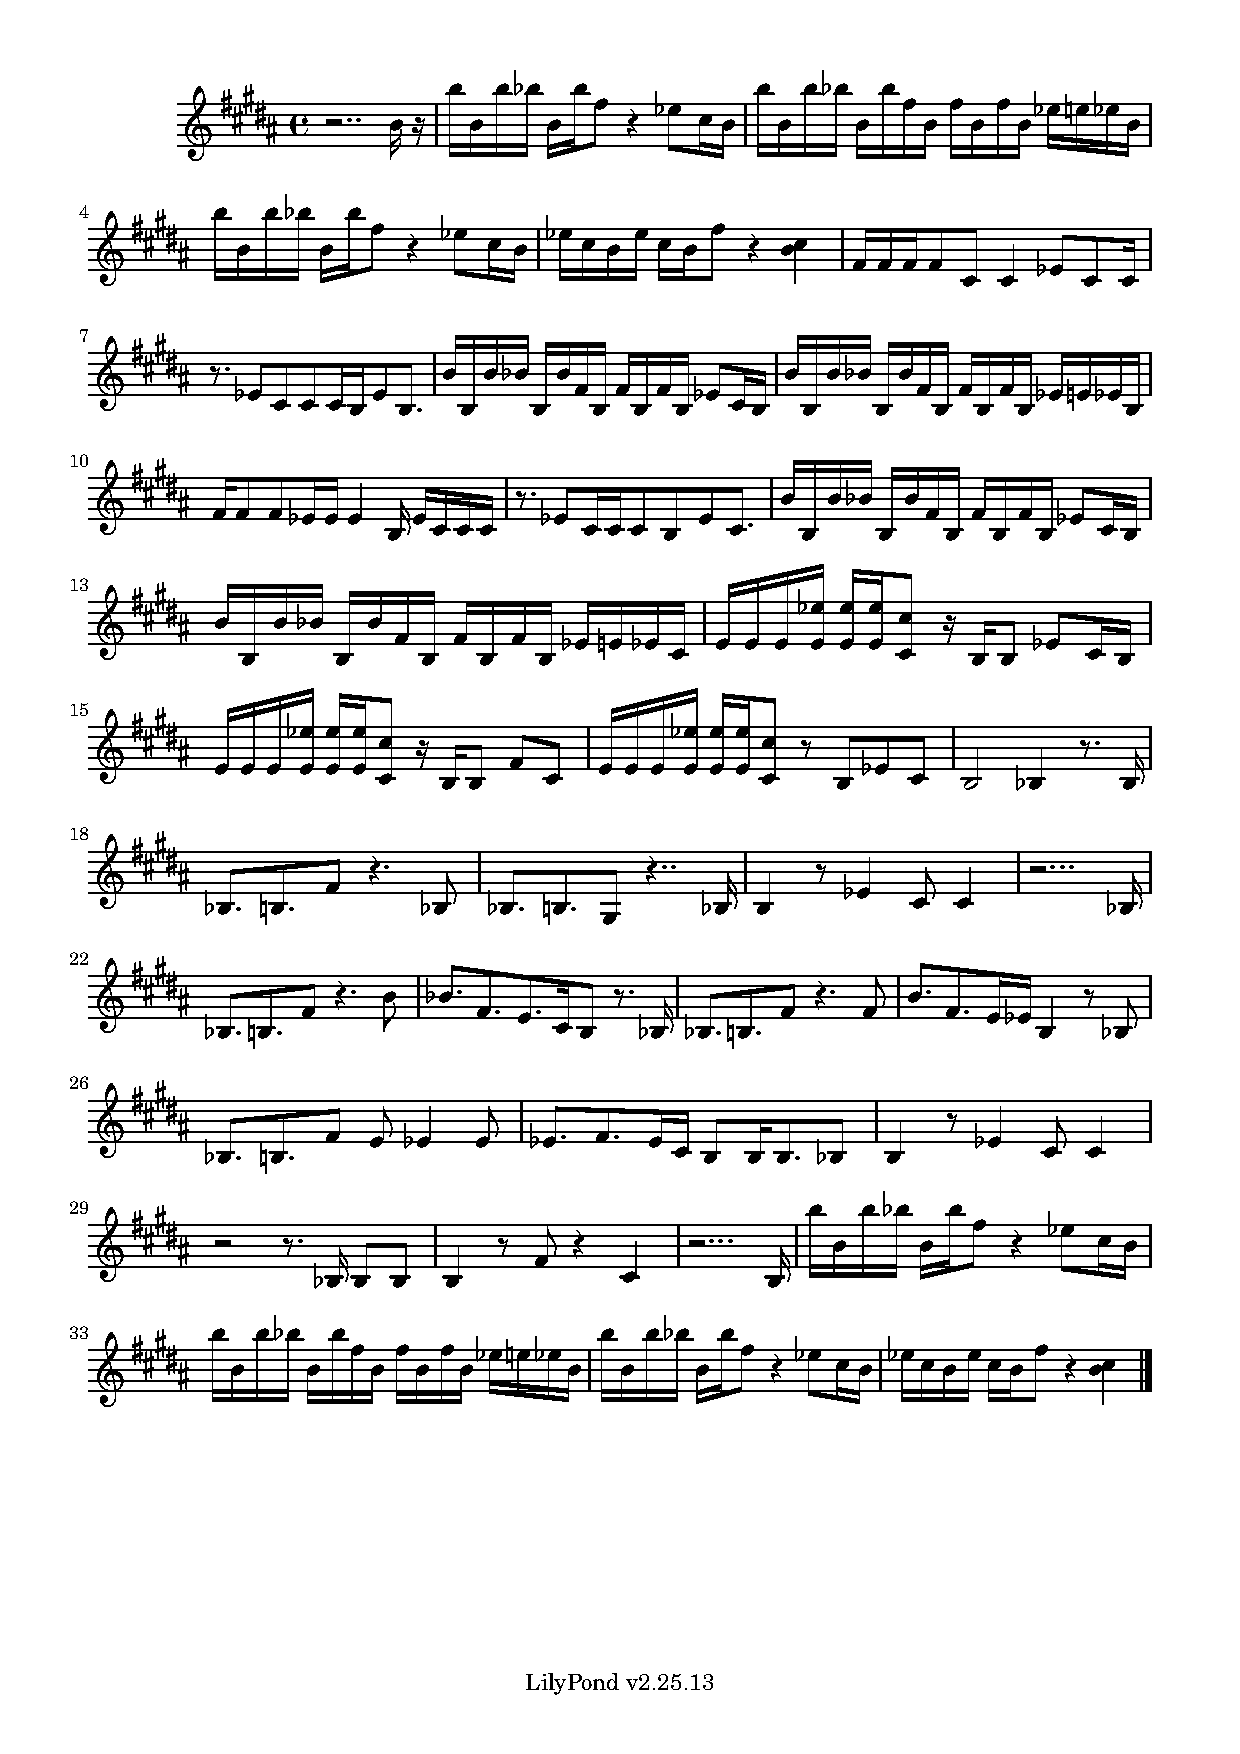
\includegraphics[trim=1cm 26.5cm 1cm 0.5cm, clip, scale=0.8]{Original_ATM.pdf}
\caption{The original notes.} 
\label{fig:OATM}
\end{subfigure}
\begin{subfigure}{\textwidth}
\centering
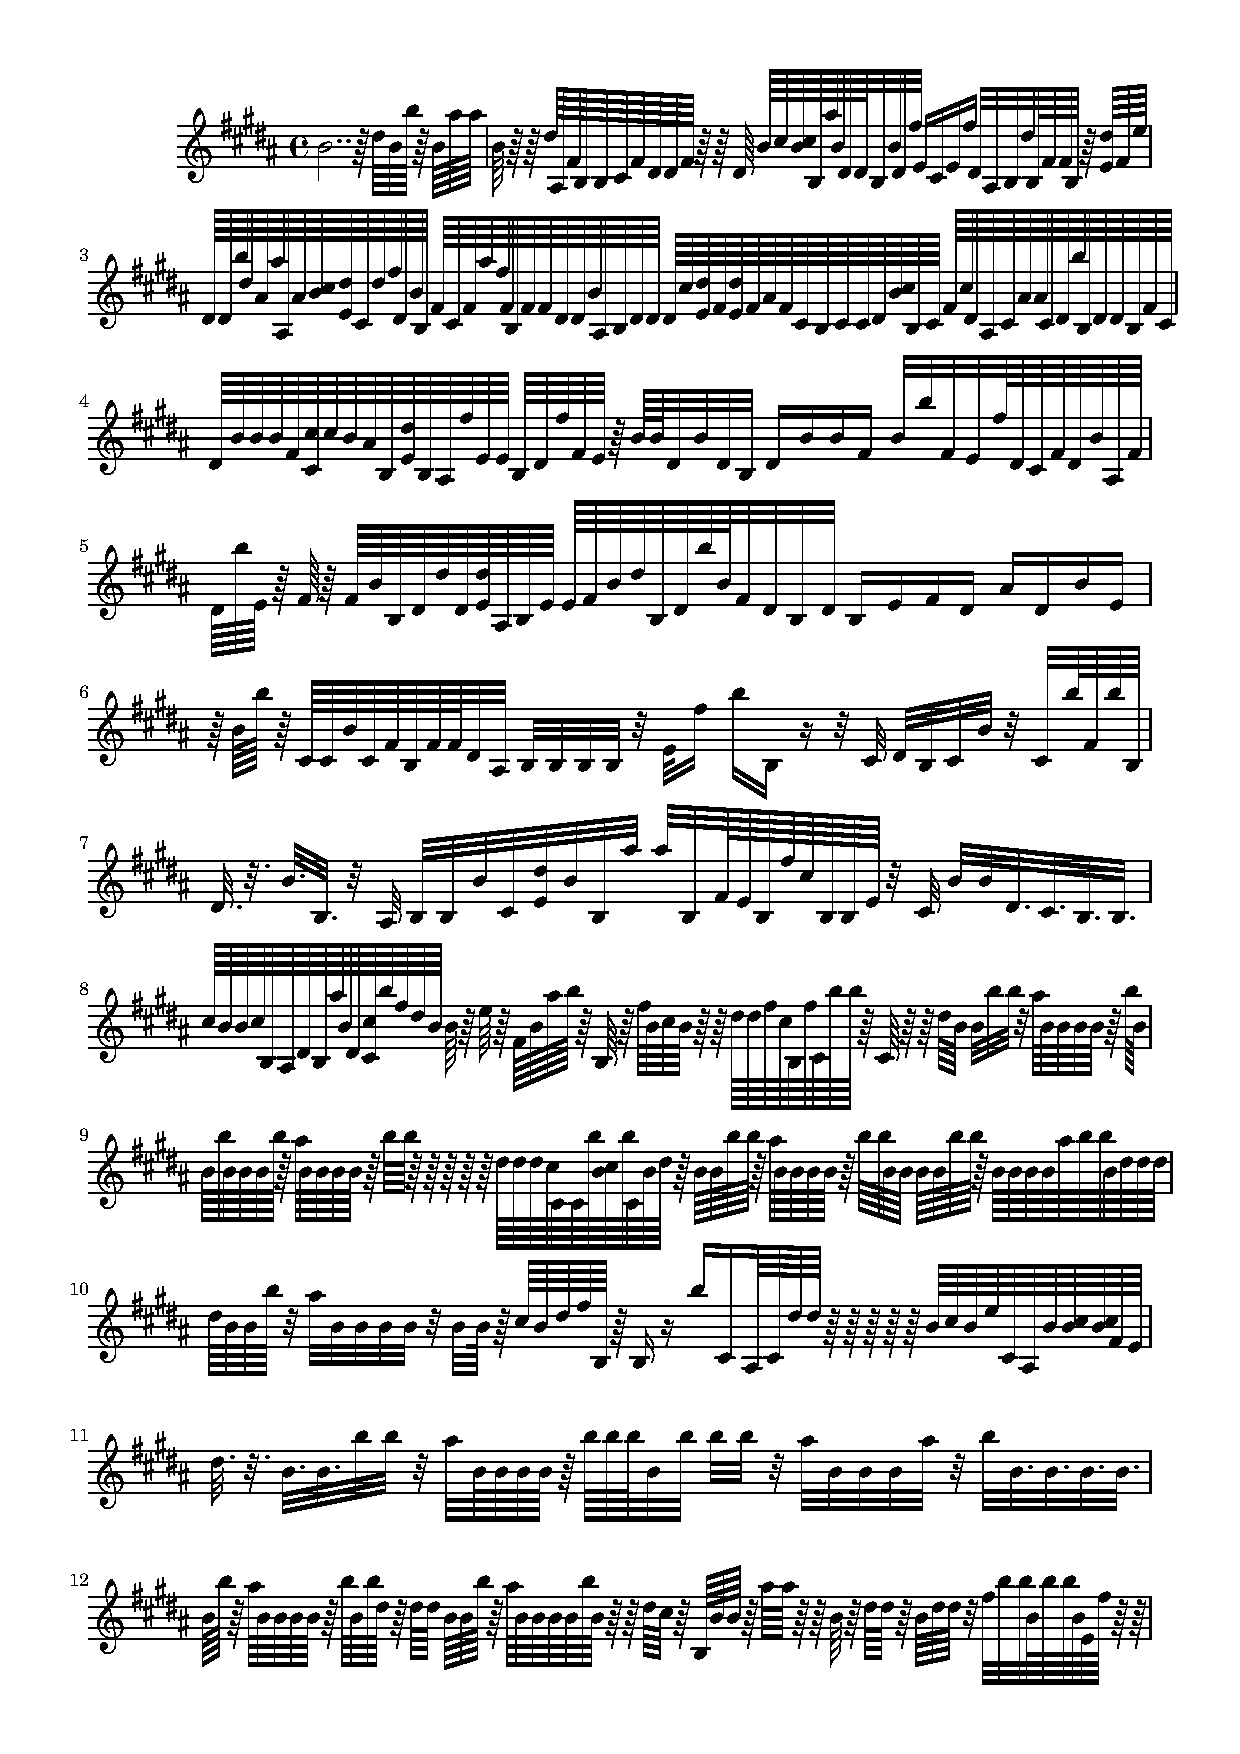
\includegraphics[trim=1cm 23.75cm 1cm 0.5cm, clip, scale=0.8]{New_ATM.pdf}
\caption{A new variation derived melodic variation with expanded rhythm.} 
\label{fig:NATM}
\end{subfigure}
\caption{The combined approach with ``A Thousand Miles" in the first 3 bars.} 
\label{fig: exam2}
\end{figure}

\subsection{Future Directions}

Exploring diverse parameters and configurations within chaotic mapping and melodic variation techniques could unlock a wider range of variation styles and outcomes, while investigating methods for user control over the variation process holds promise, enabling musicians to tailor generated variations to their specific creative goals. 
Moreover, implementing this integrated approach into music composition tools could offer composers a valuable resource for generating new musical ideas and exploring creative possibilities in a streamlined manner.

\section{Conclusion}
\label{sec: conclusion}
The proposed method, rooted in the dynamics of chaotic systems, represents an innovative approach to music composition. 
By circumventing the constraints of existing AI technologies, it empowers composers to craft compositions that are not only inventive but also rich in diversity, all while minimizing computational demands. 
This method holds the potential to ignite creativity, offering a remedy for composer burnout and ushering in an era of unprecedented musical expression fueled by chaos and innovation.

By embracing chaos as a creative force, this approach promises to redefine the landscape of music creation. 
It opens up new horizons for composers, providing them with a toolset to explore uncharted territories and break free from conventional constraints. 
As a result, this approach may hold the potential to catalyze a profound transformation in both the composition and experience of music, envisioning a future where unpredictability and diversity emerge as paramount features in musical expression.

\printbibliography

\end{document}